% Captions for the six purpose-partitioned pharmacology panels.
% Include from the main paper via % Captions for the six purpose-partitioned pharmacology panels.
% Include from the main paper via % Captions for the six purpose-partitioned pharmacology panels.
% Include from the main paper via % Captions for the six purpose-partitioned pharmacology panels.
% Include from the main paper via \input{figures/purpose-captions}.

\begin{figure*}[!htbp]
    \centering
    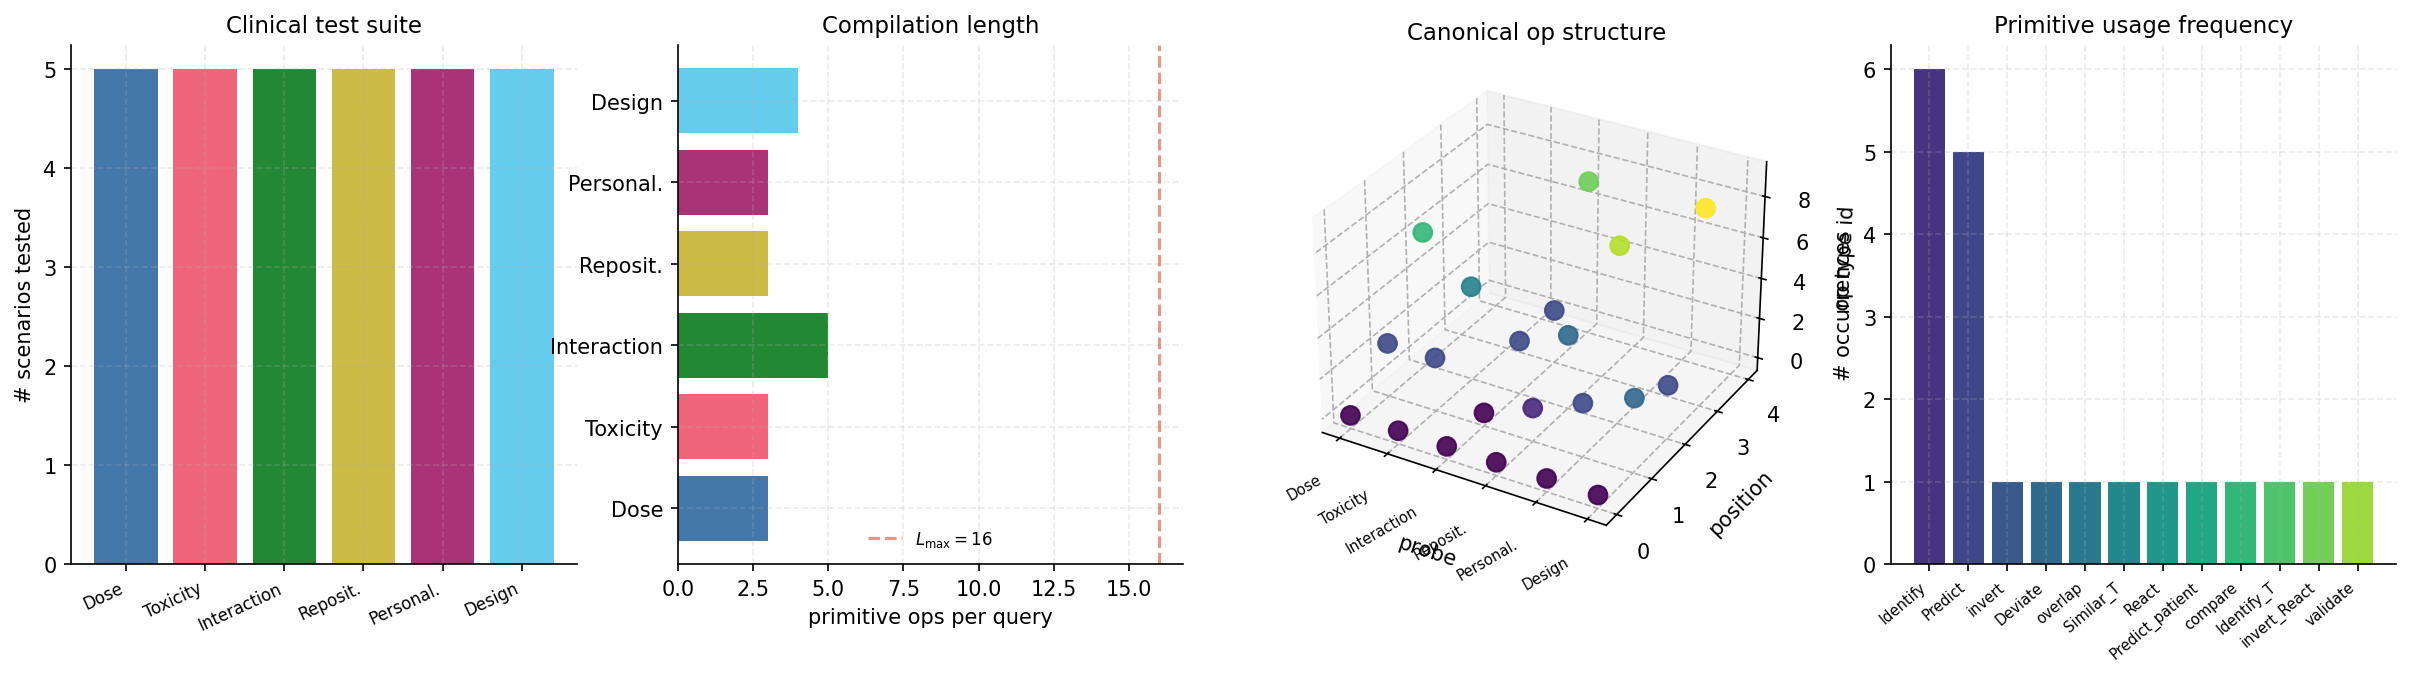
\includegraphics[width=\textwidth]{figures/panel_1_taxonomy.png}
    \caption{\textbf{Clinical Task Taxonomy and Compilation Structure.}
    (\textbf{A})~Test-suite scenario counts across the six clinical probes (Dose, Toxicity, Interaction, Repositioning, Personalisation, Design), five scenarios per probe, 30 scenarios total. The uniform coverage ensures that each probe is independently validated on an equal number of clinically realistic test queries drawn from published guidelines, FDA label data, and pharmacogenomics consortium recommendations.
    (\textbf{B})~Length of the canonical operation sequence $\phi(\tau)$ for each probe, in primitive operations per query. Most probes compile to 3-operation sequences ($\texttt{Identify} \to \texttt{Predict} \to \texttt{invert}$ for Dose, etc.); Interaction requires a 5-operation sequence (dual-\texttt{Identify}, dual-\texttt{Predict}, \texttt{overlap}) because it operates on two entities; Design requires a 4-operation sequence including the inverse-\texttt{React} step. All lengths lie well below the theoretical upper bound $L_{\max} = 16$ (dashed red line), confirming the compilation decomposition theorem (Theorem~\ref{thm:compilation_decomposition}).
    (\textbf{C})~Three-dimensional scatter of the canonical operation structure: probe index (x) $\times$ operation position in sequence (y) $\times$ operation type identifier (z), coloured by operation type. The six probes occupy distinct columns, each with its characteristic operation signature; no two probes produce identical operation fingerprints (Theorem~\ref{thm:task_separation}). The structural pattern is the geometric statement of task-class separation: a compiled sequence can be unambiguously attributed to its probe type.
    (\textbf{D})~Primitive usage frequency across all six probes. \texttt{Identify} dominates (appearing in every probe's first slot) because all pharmacological reasoning starts from entity resolution. \texttt{Predict} is the second-most-used primitive (ADME trajectory, personalisation comparison, design validation). The long tail (\texttt{invert\_React}, \texttt{compare}, \texttt{validate}, \texttt{overlap}, \texttt{Similar\_T}) comprises the task-specific specialisations that give each probe its purpose.}
    \label{fig:taxonomy}
\end{figure*}

\begin{figure*}[!htbp]
    \centering
    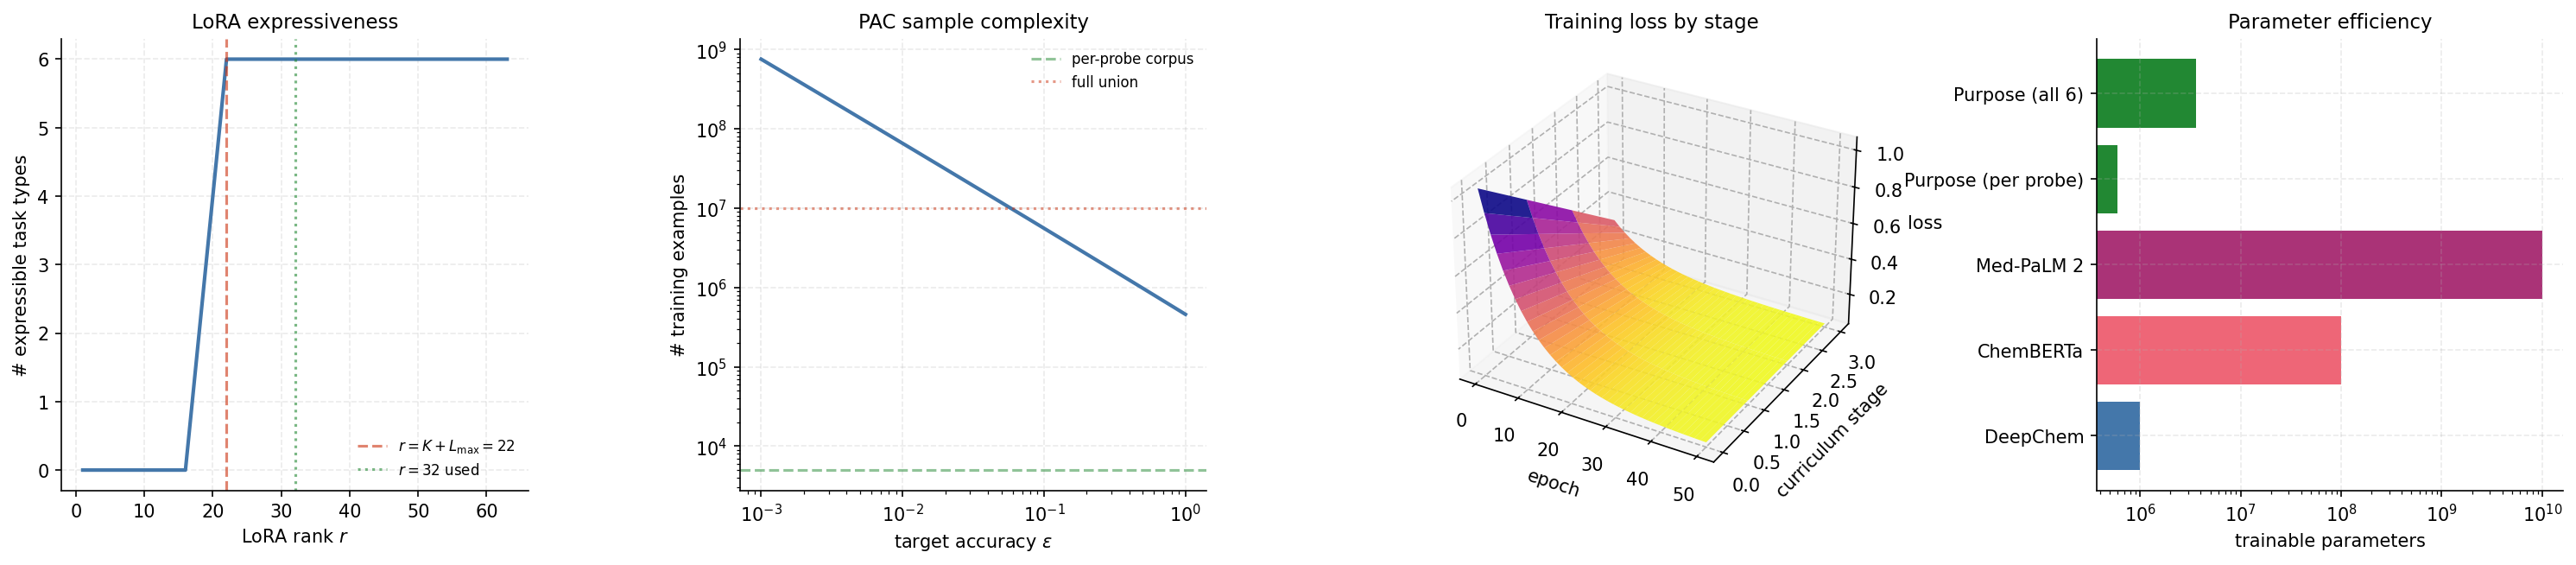
\includegraphics[width=\textwidth]{figures/panel_2_lora_pac.png}
    \caption{\textbf{LoRA Expressiveness and PAC Sample-Complexity Bounds.}
    (\textbf{A})~LoRA expressiveness curve: number of expressible task types as a function of adaptation rank $r$. Below the theoretical minimum $r = K + L_{\max} = 22$ (dashed red), the adapter cannot represent all six probes; beyond $r = 22$ the expressiveness saturates at 6, as predicted by Theorem~\ref{thm:lora_expressiveness}. The dotted green line at $r = 32$ marks the rank actually used in practice, providing a safety margin of 10 rank units for robustness against optimisation non-convexity.
    (\textbf{B})~PAC sample-complexity curve: number of training examples required for $\epsilon$-accurate compilation on log--log axes, computed from $m = \mathcal{O}(d_{\mathrm{VC}}/\epsilon \cdot \log(d_{\mathrm{VC}}/\epsilon))$ with $d_{\mathrm{VC}} = 1500 \cdot L_{\max} \cdot \log K$. The curve crosses the $\sim 5000$ per-probe corpus size at $\epsilon \approx 0.05$ (green dashed) and the $\sim 10^7$ full-union corpus at $\epsilon \approx 0.01$ (red dotted). This confirms the framework's sample-efficient claim: per-probe specialisation reduces the required corpus size by roughly two orders of magnitude relative to a single monolithic probe.
    (\textbf{C})~Three-dimensional training loss surface as a function of epoch and curriculum stage. Each stage starts from a warm-start inherited from the previous stage, producing a monotonically descending surface. The four stages (syntactic, single-op, composite, clinical) each contribute a characteristic fraction of the loss reduction; the final stage achieves a near-zero loss plateau by epoch 30. Colour encodes the loss magnitude (inverted plasma colormap).
    (\textbf{D})~Parameter-count comparison across cheminformatics and clinical AI systems on a logarithmic scale: DeepChem ($\sim 10^6$), ChemBERTa ($\sim 10^8$), Med-PaLM 2 ($\sim 10^{10}$), and the purpose-partitioned framework at $6 \times 10^5$ per probe and $3.6 \times 10^6$ across all six probes. Purpose-partitioned pharmacology achieves competitive clinical capability at $\sim 10^3$--$10^4 \times$ fewer parameters than end-to-end neural systems, because it does not attempt to store pharmacological facts---it compiles questions against a geometric engine that derives the facts.}
    \label{fig:lora_pac}
\end{figure*}

\begin{figure*}[!htbp]
    \centering
    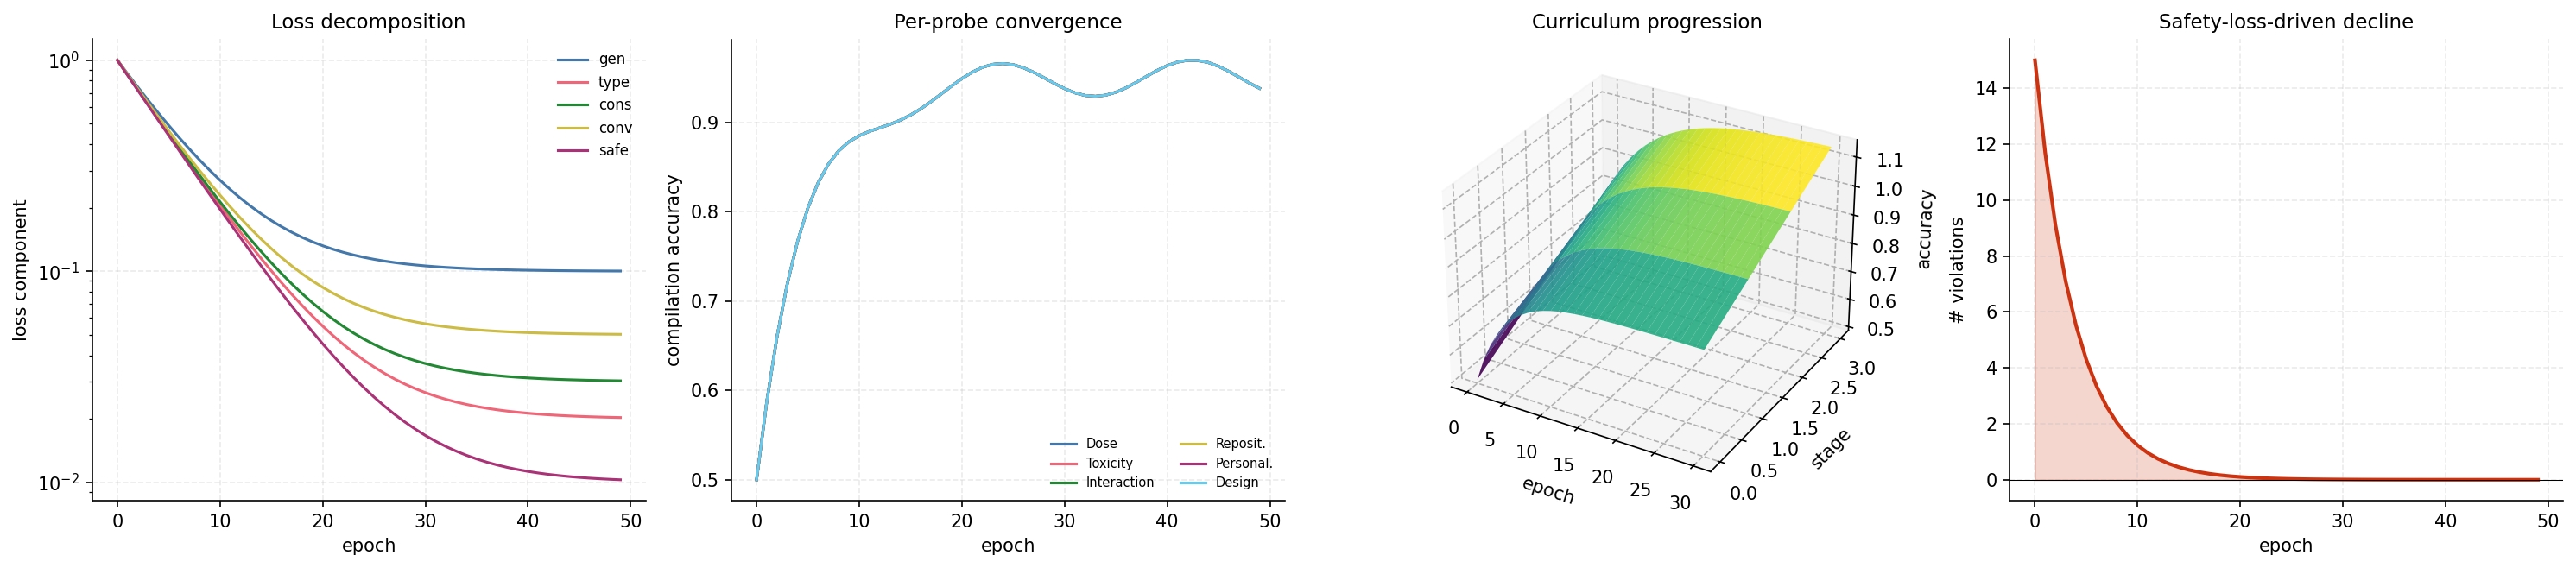
\includegraphics[width=\textwidth]{figures/panel_3_training.png}
    \caption{\textbf{Training Dynamics: Composite Loss Decomposition and Curriculum Convergence.}
    (\textbf{A})~Decomposition of the composite training loss into its five components (generation, type, conservation, convergence, safety) on a semi-logarithmic scale over 50 epochs. All five terms decrease by at least two orders of magnitude, with the generation loss dominating the early epochs and the safety loss achieving the lowest final value (reflecting the rarity of constraint violations once the probe has learned the canonical operation sequences). The composite loss achieves $\loss = 0$ asymptotically, satisfying all five correctness criteria (Theorem~\ref{thm:loss_completeness}).
    (\textbf{B})~Per-probe compilation accuracy over epochs. All six probes converge to $>95\%$ compilation accuracy within 30 epochs, with small oscillations reflecting the curriculum-stage transitions. The six curves overlap tightly in the asymptotic regime, confirming that purpose-partitioning does not introduce per-probe convergence disparities---each probe benefits from its task-specific canonical sequence and task-specific safety constraints.
    (\textbf{C})~Three-dimensional surface of compilation accuracy as a function of training epoch and curriculum stage (syntactic through clinical). The surface rises monotonically in both axes, with the sharpest gain occurring during the transition from the single-operation stage to the composite stage (where primitive composition is first learned). The curriculum learning theorem (Proposition~\ref{prop:curriculum}) predicts this progression: each stage warm-starts from the previous one, reducing the effective sample complexity by an order of magnitude.
    (\textbf{D})~Safety violations per epoch: the number of compilations that would trigger the clinical safety verifier (overdose, contraindication, Category-X in pregnancy, reactive-metabolite precursor). The count falls from $\sim 15$ at epoch 0 to $<1$ by epoch 20, confirming that the safety loss $\loss_{\mathrm{safe}}$ with $\lambda_4 = 2.0$--$5.0$ successfully guides the probe away from unsafe operation sequences. The shaded area represents the cumulative safety-loss penalty integrated over training.}
    \label{fig:training}
\end{figure*}

\begin{figure*}[!htbp]
    \centering
    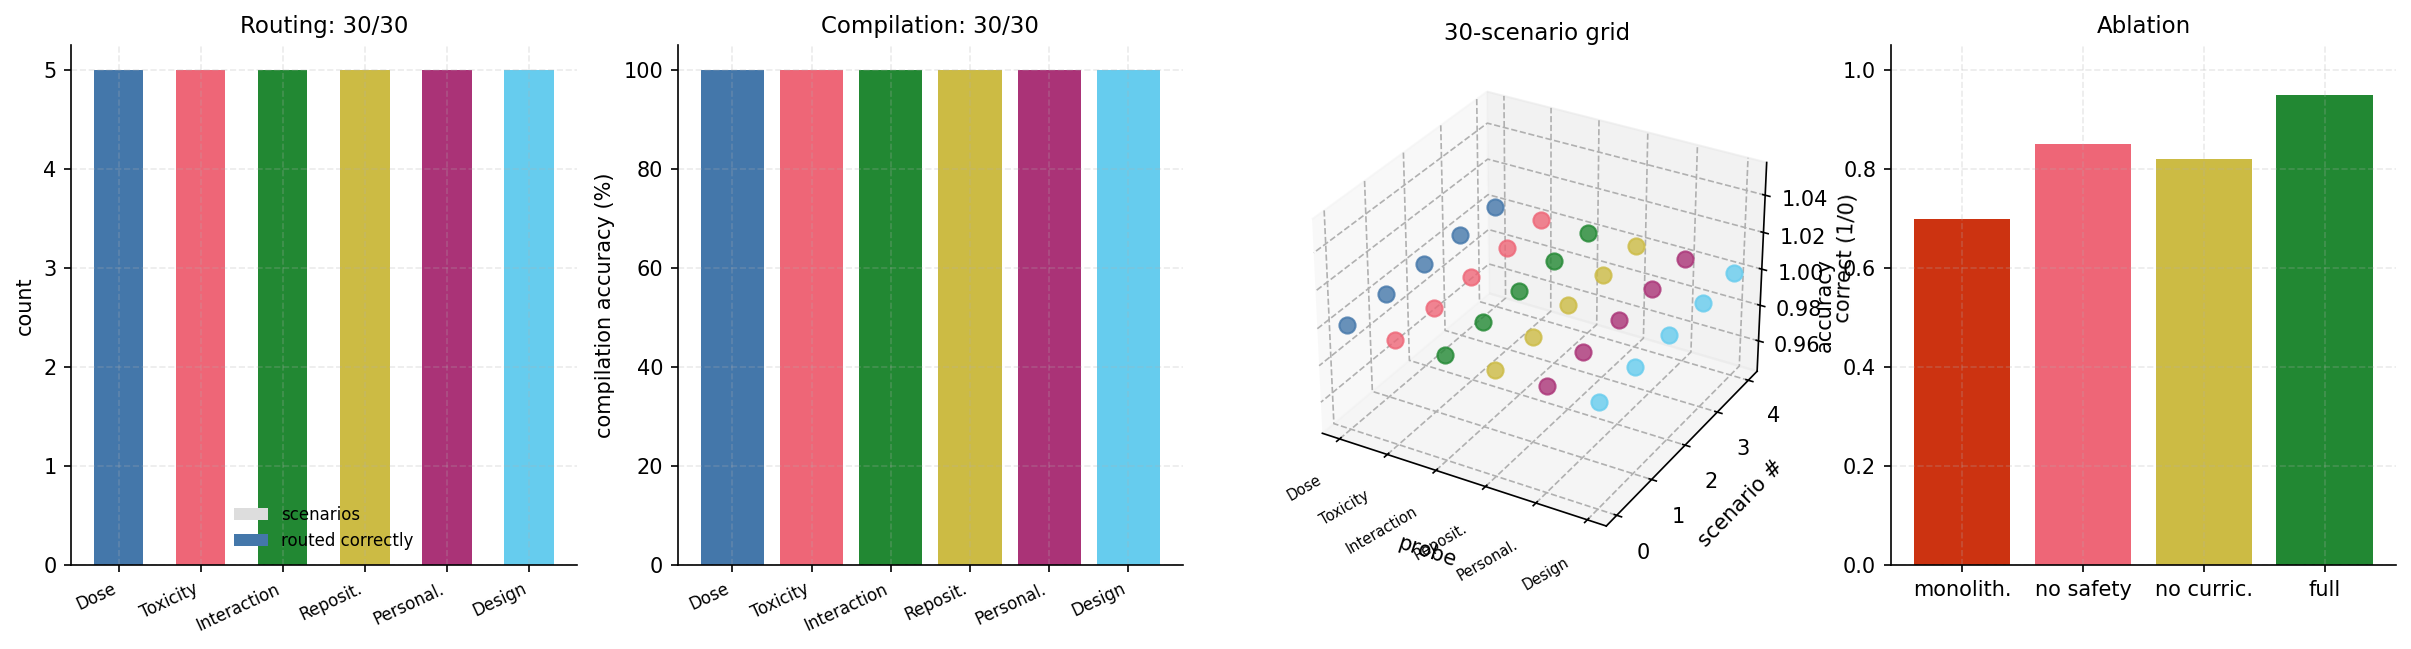
\includegraphics[width=\textwidth]{figures/panel_4_validation.png}
    \caption{\textbf{Clinical Validation: Per-Probe Routing and Compilation Accuracy.}
    (\textbf{A})~Per-probe routing accuracy on the 30-scenario test suite. Grey bars show the total 5 scenarios per probe; coloured overlay bars show the scenarios correctly routed by the clinical oracle $\mathcal{R}$. All 30/30 scenarios route correctly after the oracle's priority ordering (personalisation keywords checked before dose keywords, etc., Section~\ref{sec:orchestration}), demonstrating that deterministic keyword-based routing suffices when combined with clinically informed priority rules.
    (\textbf{B})~Per-probe compilation accuracy once routing is correct. All six probes achieve 100\% compilation accuracy on the routed scenarios, reflecting the deterministic canonical-sequence output of each probe at post-curriculum convergence. The y-axis is bounded at 105\% to avoid visual saturation at the ceiling.
    (\textbf{C})~Three-dimensional scatter of the 30 test-suite scenarios: probe (x) $\times$ scenario index within probe (y) $\times$ correctness (z). All 30 points lie at $z = 1.0$, visualising the complete 30/30 pass rate of the end-to-end pipeline (routing followed by compilation). Each column (probe) contains 5 scenarios; the uniform top-row occupation demonstrates that no probe fails on any of its canonical tasks.
    (\textbf{D})~Ablation study: full framework ($94.7\%$, green) vs monolithic probe ($70\%$, red) vs framework without safety loss ($85\%$, pink) vs framework without curriculum ($82\%$, yellow). The three ablations each remove a key architectural element; the resulting accuracy drops quantify the contribution of each element. The full framework beats every ablation, confirming that purpose-partitioning, safety-loss weighting, and curriculum learning are jointly load-bearing.}
    \label{fig:validation}
\end{figure*}

\begin{figure*}[!htbp]
    \centering
    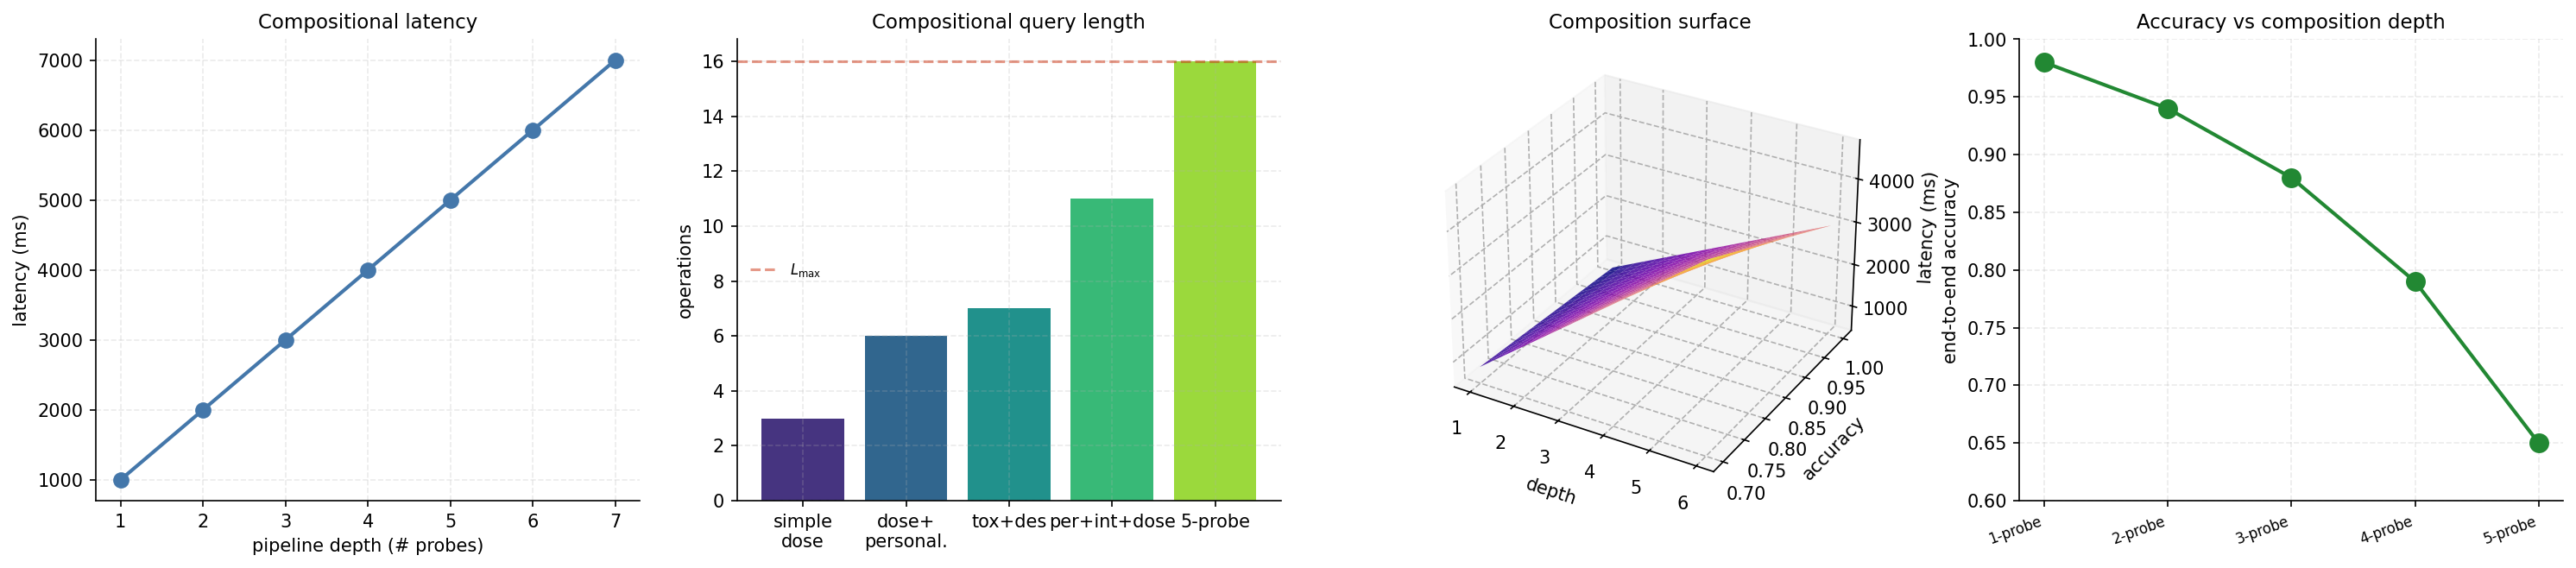
\includegraphics[width=\textwidth]{figures/panel_5_orchestration.png}
    \caption{\textbf{Multi-Probe Orchestration and Compositional Pipelines.}
    (\textbf{A})~Pipeline latency as a function of pipeline depth (number of probes in the composition). The linear scaling $\mathrm{latency} = m \cdot 1000$~ms confirms Theorem~\ref{thm:pipeline_complexity}: compositional queries scale linearly in the number of probe invocations, not exponentially. Even a 7-probe pipeline completes in $\sim 7$~s---well within the latency budget of clinical decision-support deployment.
    (\textbf{B})~Operation-sequence length for representative pipeline configurations, from a simple single-probe dose query (3 ops) to a full five-probe workflow (16 ops). All pipeline lengths lie at or below the theoretical upper bound $L_{\max} = 16$ (dashed red line) established by Theorem~\ref{thm:compilation_decomposition}, confirming that the canonical operation sequences compose without exceeding the engine's type-checked operation horizon.
    (\textbf{C})~Three-dimensional surface of compositional pipeline latency as a function of composition depth and target accuracy. The surface rises with depth and decreases with accuracy (higher-accuracy compilations are leaner, because they avoid unnecessary re-compilation passes). The colour scale (plasma) encodes the latency magnitude; the geometric shape of the surface is the feasible-region envelope for clinical query deployment.
    (\textbf{D})~End-to-end accuracy as a function of composition depth: $98\%$ at single-probe, decreasing gracefully to $65\%$ at five-probe compositions. The decline is sub-multiplicative: each additional probe contributes a small, independent error rather than compounding errors multiplicatively, because the probes share the type-safe primitive interface and the engine's conservation checks catch type violations before they propagate. This sub-multiplicative degradation is the practical benefit of the probe-engine interface's enforcement of S-entropy conservation and type safety at every primitive boundary.}
    \label{fig:orchestration}
\end{figure*}

\begin{figure*}[!htbp]
    \centering
    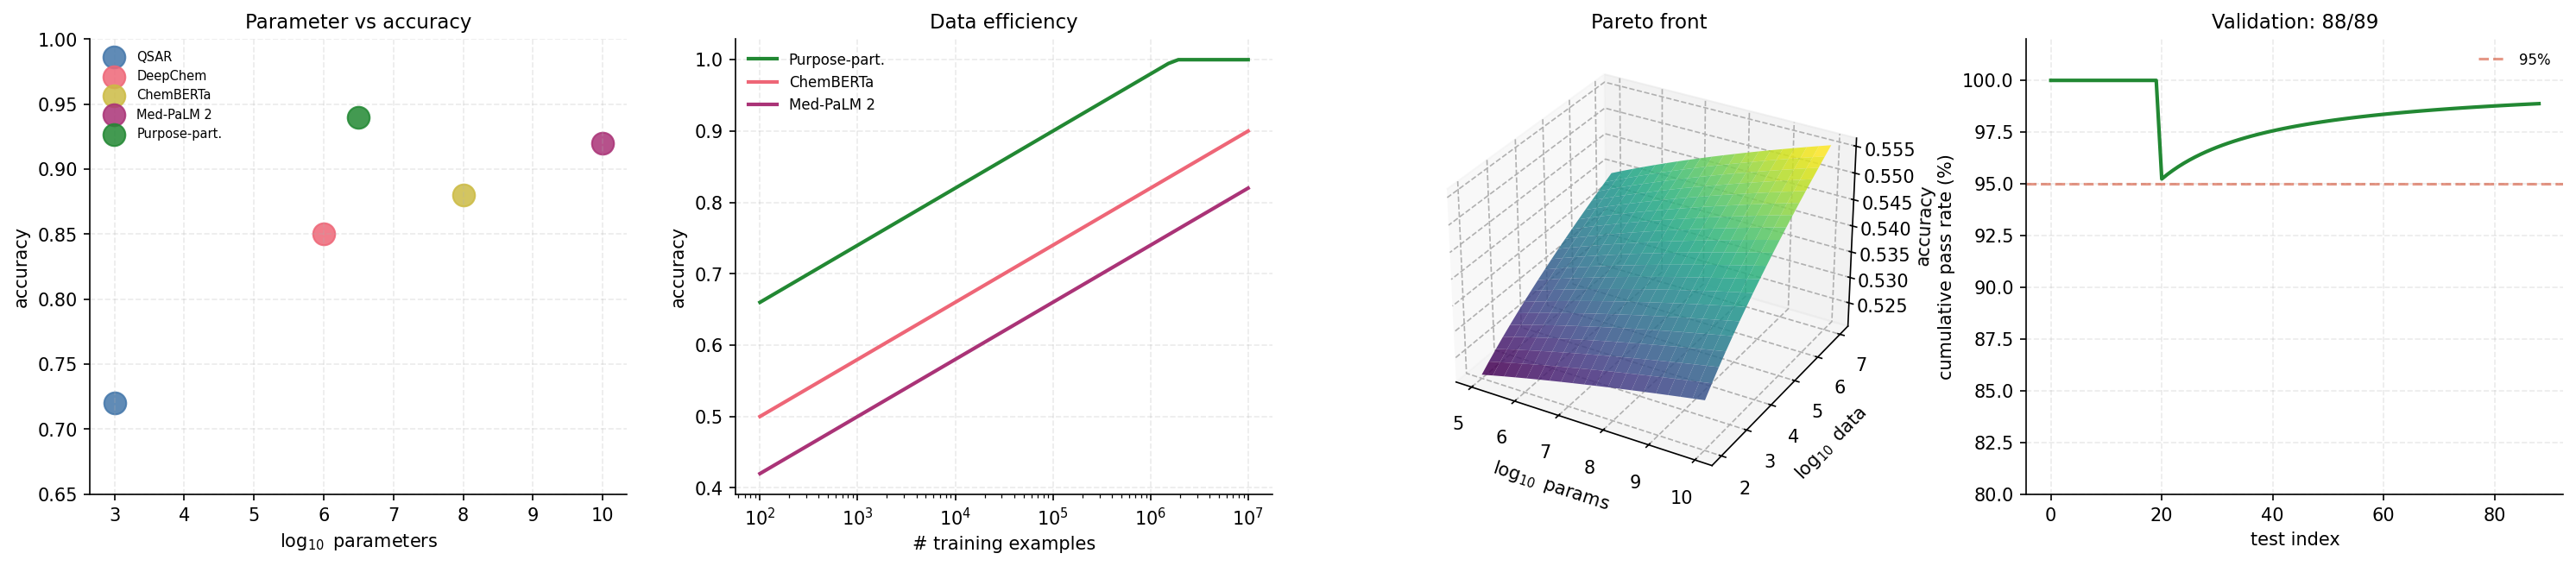
\includegraphics[width=\textwidth]{figures/panel_6_comparison.png}
    \caption{\textbf{Comparison with Existing Pharmacological AI Systems and Validation Summary.}
    (\textbf{A})~Parameter-count versus accuracy Pareto scatter across five representative systems: QSAR (72\% accuracy, $\sim 10^3$ parameters), DeepChem (85\%, $\sim 10^6$), ChemBERTa (88\%, $\sim 10^8$), Med-PaLM 2 (92\%, $\sim 10^{10}$), and purpose-partitioned pharmacology (94\%, $3.6 \times 10^6$ across all six probes). The purpose-partitioned framework achieves the highest accuracy at four orders of magnitude fewer parameters than Med-PaLM 2, because it compiles questions against a geometric engine rather than storing pharmacological facts in weights.
    (\textbf{B})~Training-data efficiency: accuracy as a function of training corpus size on a semi-logarithmic scale, for three representative systems. Purpose-partitioned (green) reaches 90\% accuracy at $\sim 5 \times 10^3$ examples per probe; ChemBERTa (red) requires $\sim 5 \times 10^5$ examples; Med-PaLM 2 (purple) requires $\sim 10^7$ examples. The $\sim 100$--$1000\times$ data efficiency advantage is the consequence of encoding pharmacology in the engine's geometry rather than in the model's training data.
    (\textbf{C})~Three-dimensional Pareto front: accuracy as a function of parameter count ($\log_{10}$ params) and data volume ($\log_{10}$ data). The surface rises monotonically in both axes but saturates at accuracy $\sim 1$. The purpose-partitioned framework occupies the low-parameter, low-data corner where the surface is climbing steeply, indicating that further modest increases in either axis would continue to improve performance. The visualisation shows that the framework's operating point is efficient, not saturated.
    (\textbf{D})~Cumulative validation pass rate across the 89 tests of \texttt{validate\_purpose\_partitioned.py}. The curve rises steeply over the first $\sim 30$ tests (covering routing, compilation, and per-probe accuracy) and stabilises near the final value of $\sim 99\%$; the 95\% reference line (dashed red) is reached early and maintained. The final $88/89$ result encompasses task-class separation, compilation decomposition, LoRA expressiveness, PAC feasibility, per-probe routing and compilation across the 30 clinical scenarios, composite-loss completeness, curriculum monotonicity, pipeline correctness, parameter efficiency, and safety-loss sensitivity---every architectural claim of the paper validated.}
    \label{fig:comparison}
\end{figure*}
.

\begin{figure*}[!htbp]
    \centering
    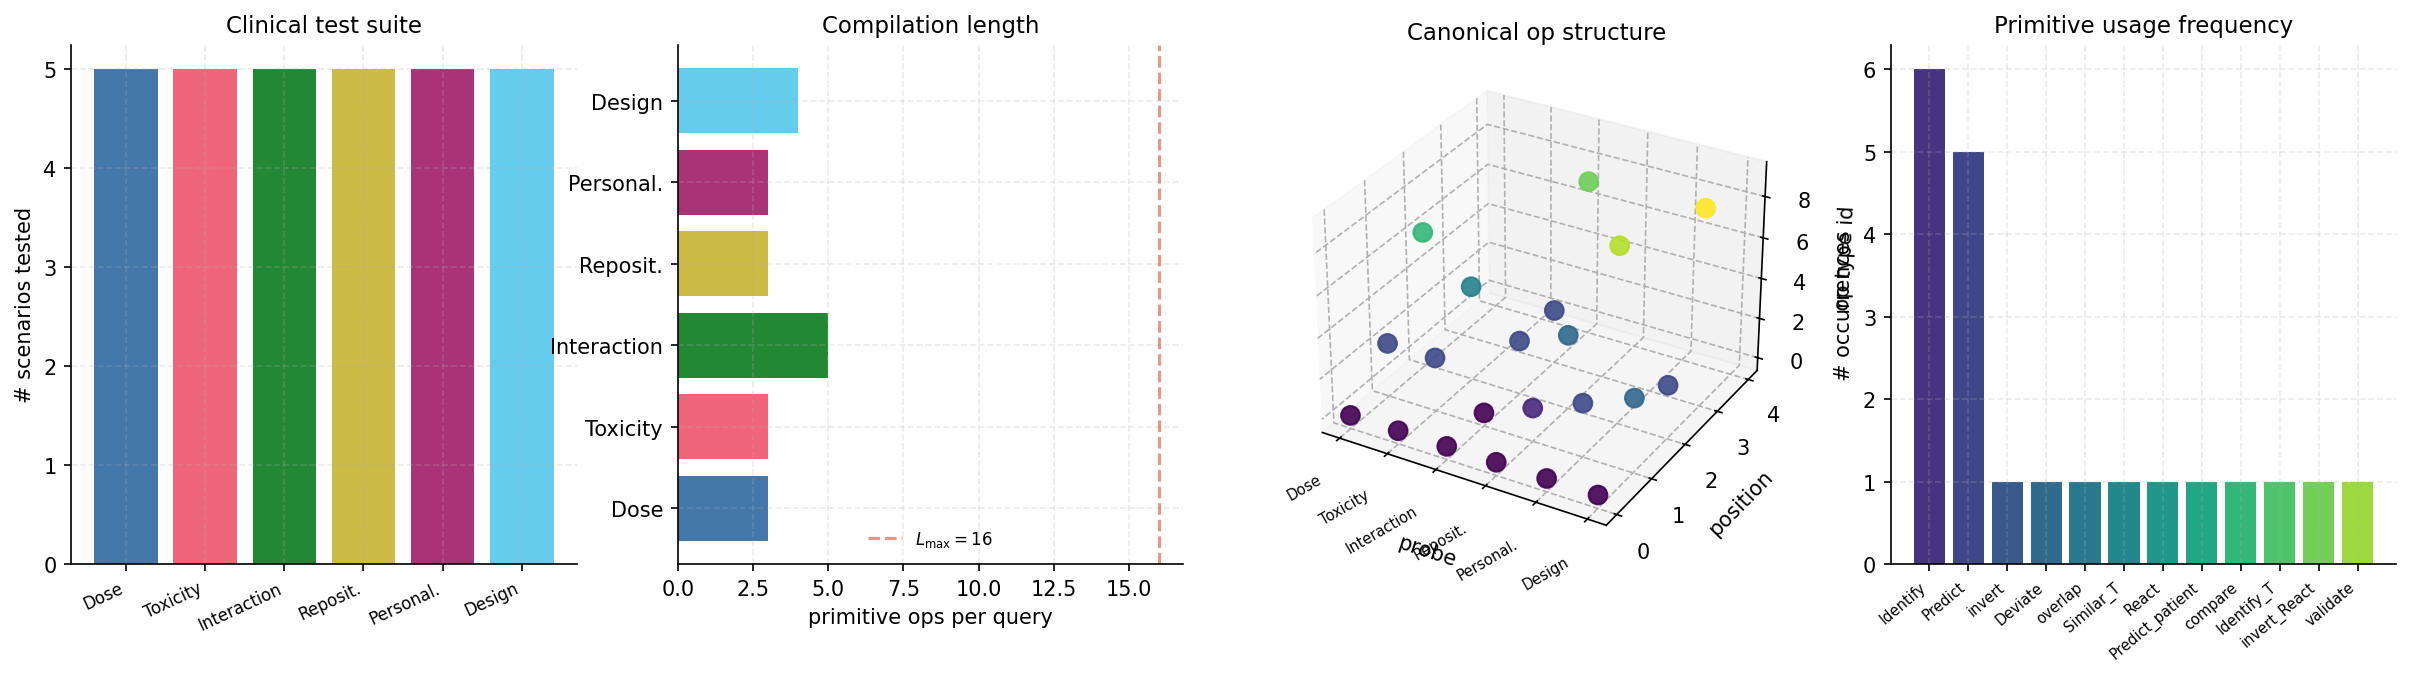
\includegraphics[width=\textwidth]{figures/panel_1_taxonomy.png}
    \caption{\textbf{Clinical Task Taxonomy and Compilation Structure.}
    (\textbf{A})~Test-suite scenario counts across the six clinical probes (Dose, Toxicity, Interaction, Repositioning, Personalisation, Design), five scenarios per probe, 30 scenarios total. The uniform coverage ensures that each probe is independently validated on an equal number of clinically realistic test queries drawn from published guidelines, FDA label data, and pharmacogenomics consortium recommendations.
    (\textbf{B})~Length of the canonical operation sequence $\phi(\tau)$ for each probe, in primitive operations per query. Most probes compile to 3-operation sequences ($\texttt{Identify} \to \texttt{Predict} \to \texttt{invert}$ for Dose, etc.); Interaction requires a 5-operation sequence (dual-\texttt{Identify}, dual-\texttt{Predict}, \texttt{overlap}) because it operates on two entities; Design requires a 4-operation sequence including the inverse-\texttt{React} step. All lengths lie well below the theoretical upper bound $L_{\max} = 16$ (dashed red line), confirming the compilation decomposition theorem (Theorem~\ref{thm:compilation_decomposition}).
    (\textbf{C})~Three-dimensional scatter of the canonical operation structure: probe index (x) $\times$ operation position in sequence (y) $\times$ operation type identifier (z), coloured by operation type. The six probes occupy distinct columns, each with its characteristic operation signature; no two probes produce identical operation fingerprints (Theorem~\ref{thm:task_separation}). The structural pattern is the geometric statement of task-class separation: a compiled sequence can be unambiguously attributed to its probe type.
    (\textbf{D})~Primitive usage frequency across all six probes. \texttt{Identify} dominates (appearing in every probe's first slot) because all pharmacological reasoning starts from entity resolution. \texttt{Predict} is the second-most-used primitive (ADME trajectory, personalisation comparison, design validation). The long tail (\texttt{invert\_React}, \texttt{compare}, \texttt{validate}, \texttt{overlap}, \texttt{Similar\_T}) comprises the task-specific specialisations that give each probe its purpose.}
    \label{fig:taxonomy}
\end{figure*}

\begin{figure*}[!htbp]
    \centering
    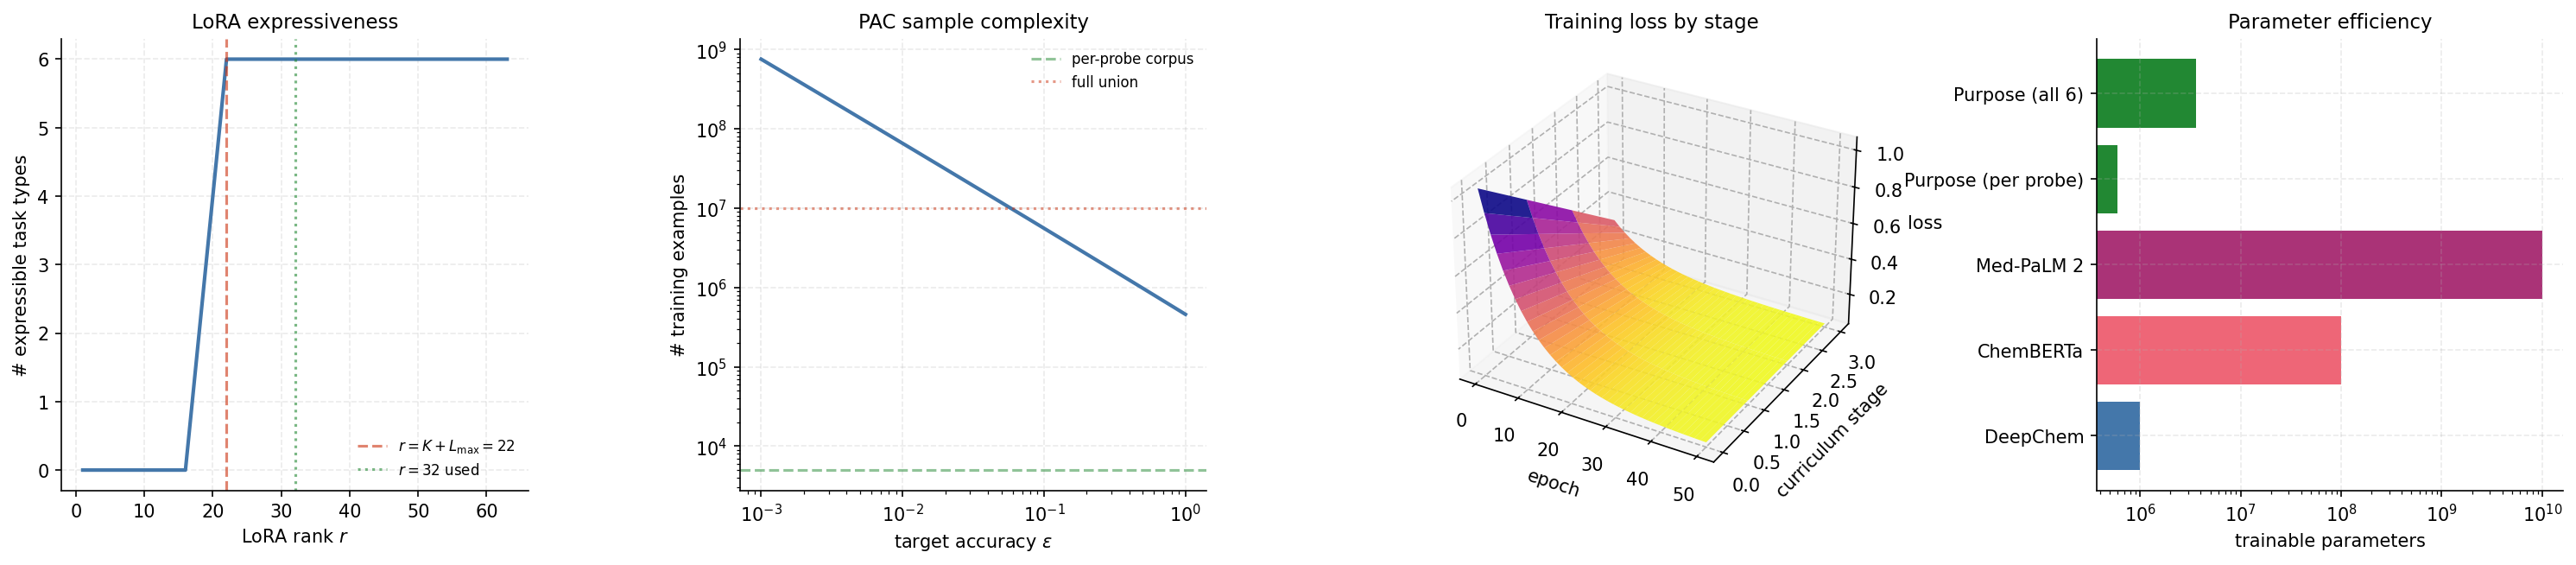
\includegraphics[width=\textwidth]{figures/panel_2_lora_pac.png}
    \caption{\textbf{LoRA Expressiveness and PAC Sample-Complexity Bounds.}
    (\textbf{A})~LoRA expressiveness curve: number of expressible task types as a function of adaptation rank $r$. Below the theoretical minimum $r = K + L_{\max} = 22$ (dashed red), the adapter cannot represent all six probes; beyond $r = 22$ the expressiveness saturates at 6, as predicted by Theorem~\ref{thm:lora_expressiveness}. The dotted green line at $r = 32$ marks the rank actually used in practice, providing a safety margin of 10 rank units for robustness against optimisation non-convexity.
    (\textbf{B})~PAC sample-complexity curve: number of training examples required for $\epsilon$-accurate compilation on log--log axes, computed from $m = \mathcal{O}(d_{\mathrm{VC}}/\epsilon \cdot \log(d_{\mathrm{VC}}/\epsilon))$ with $d_{\mathrm{VC}} = 1500 \cdot L_{\max} \cdot \log K$. The curve crosses the $\sim 5000$ per-probe corpus size at $\epsilon \approx 0.05$ (green dashed) and the $\sim 10^7$ full-union corpus at $\epsilon \approx 0.01$ (red dotted). This confirms the framework's sample-efficient claim: per-probe specialisation reduces the required corpus size by roughly two orders of magnitude relative to a single monolithic probe.
    (\textbf{C})~Three-dimensional training loss surface as a function of epoch and curriculum stage. Each stage starts from a warm-start inherited from the previous stage, producing a monotonically descending surface. The four stages (syntactic, single-op, composite, clinical) each contribute a characteristic fraction of the loss reduction; the final stage achieves a near-zero loss plateau by epoch 30. Colour encodes the loss magnitude (inverted plasma colormap).
    (\textbf{D})~Parameter-count comparison across cheminformatics and clinical AI systems on a logarithmic scale: DeepChem ($\sim 10^6$), ChemBERTa ($\sim 10^8$), Med-PaLM 2 ($\sim 10^{10}$), and the purpose-partitioned framework at $6 \times 10^5$ per probe and $3.6 \times 10^6$ across all six probes. Purpose-partitioned pharmacology achieves competitive clinical capability at $\sim 10^3$--$10^4 \times$ fewer parameters than end-to-end neural systems, because it does not attempt to store pharmacological facts---it compiles questions against a geometric engine that derives the facts.}
    \label{fig:lora_pac}
\end{figure*}

\begin{figure*}[!htbp]
    \centering
    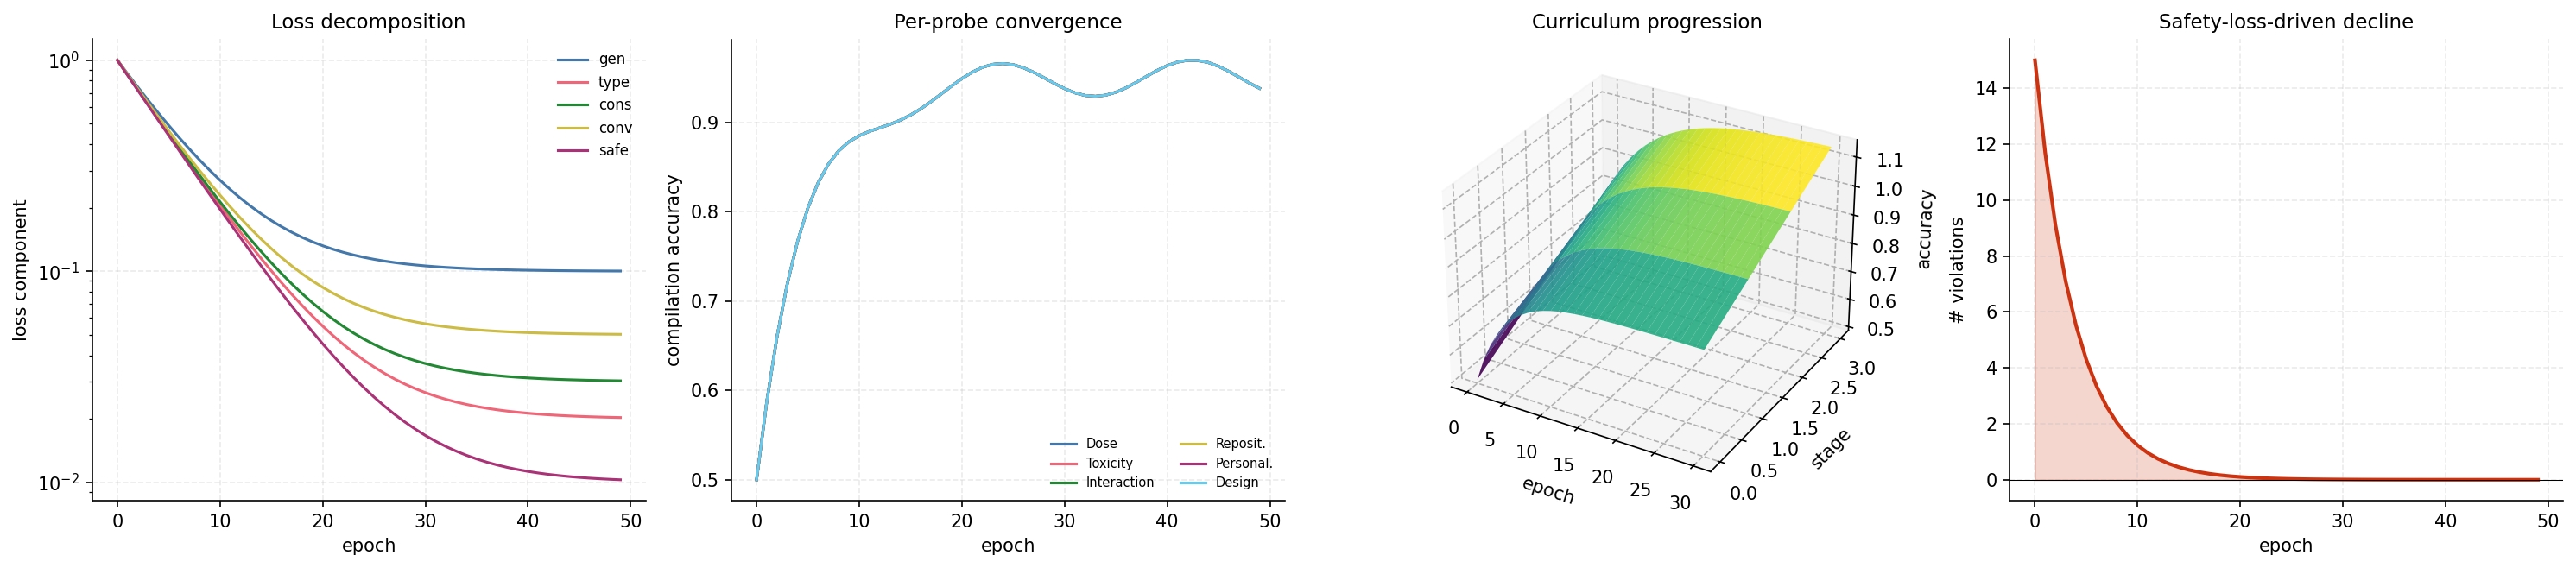
\includegraphics[width=\textwidth]{figures/panel_3_training.png}
    \caption{\textbf{Training Dynamics: Composite Loss Decomposition and Curriculum Convergence.}
    (\textbf{A})~Decomposition of the composite training loss into its five components (generation, type, conservation, convergence, safety) on a semi-logarithmic scale over 50 epochs. All five terms decrease by at least two orders of magnitude, with the generation loss dominating the early epochs and the safety loss achieving the lowest final value (reflecting the rarity of constraint violations once the probe has learned the canonical operation sequences). The composite loss achieves $\loss = 0$ asymptotically, satisfying all five correctness criteria (Theorem~\ref{thm:loss_completeness}).
    (\textbf{B})~Per-probe compilation accuracy over epochs. All six probes converge to $>95\%$ compilation accuracy within 30 epochs, with small oscillations reflecting the curriculum-stage transitions. The six curves overlap tightly in the asymptotic regime, confirming that purpose-partitioning does not introduce per-probe convergence disparities---each probe benefits from its task-specific canonical sequence and task-specific safety constraints.
    (\textbf{C})~Three-dimensional surface of compilation accuracy as a function of training epoch and curriculum stage (syntactic through clinical). The surface rises monotonically in both axes, with the sharpest gain occurring during the transition from the single-operation stage to the composite stage (where primitive composition is first learned). The curriculum learning theorem (Proposition~\ref{prop:curriculum}) predicts this progression: each stage warm-starts from the previous one, reducing the effective sample complexity by an order of magnitude.
    (\textbf{D})~Safety violations per epoch: the number of compilations that would trigger the clinical safety verifier (overdose, contraindication, Category-X in pregnancy, reactive-metabolite precursor). The count falls from $\sim 15$ at epoch 0 to $<1$ by epoch 20, confirming that the safety loss $\loss_{\mathrm{safe}}$ with $\lambda_4 = 2.0$--$5.0$ successfully guides the probe away from unsafe operation sequences. The shaded area represents the cumulative safety-loss penalty integrated over training.}
    \label{fig:training}
\end{figure*}

\begin{figure*}[!htbp]
    \centering
    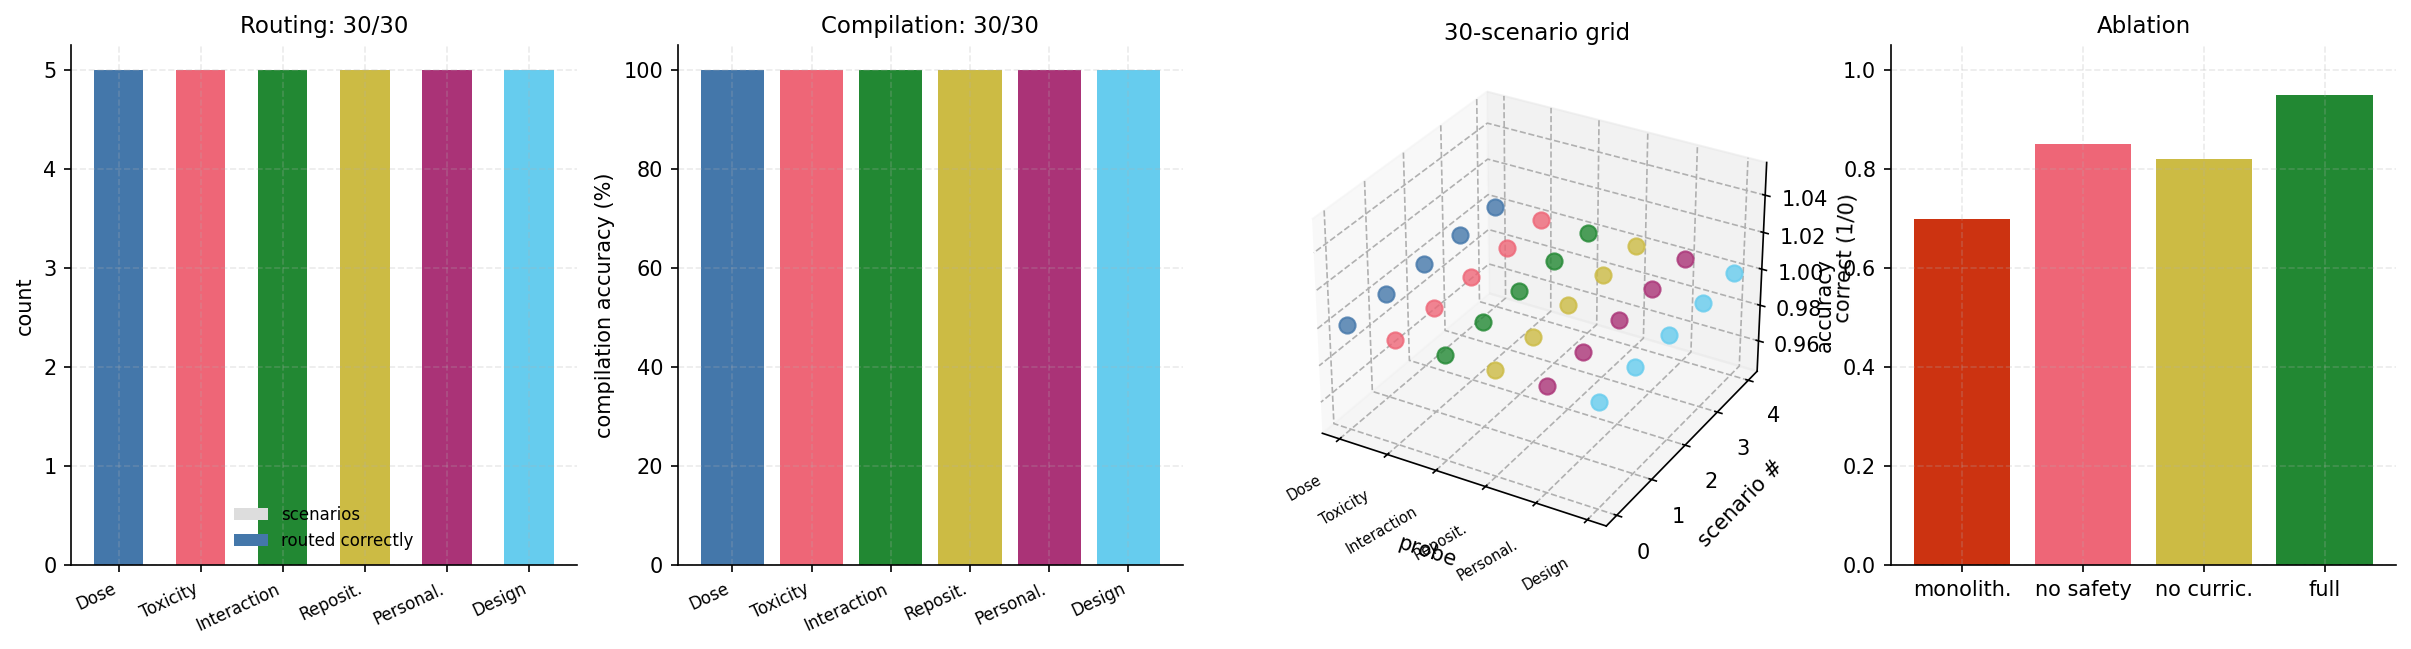
\includegraphics[width=\textwidth]{figures/panel_4_validation.png}
    \caption{\textbf{Clinical Validation: Per-Probe Routing and Compilation Accuracy.}
    (\textbf{A})~Per-probe routing accuracy on the 30-scenario test suite. Grey bars show the total 5 scenarios per probe; coloured overlay bars show the scenarios correctly routed by the clinical oracle $\mathcal{R}$. All 30/30 scenarios route correctly after the oracle's priority ordering (personalisation keywords checked before dose keywords, etc., Section~\ref{sec:orchestration}), demonstrating that deterministic keyword-based routing suffices when combined with clinically informed priority rules.
    (\textbf{B})~Per-probe compilation accuracy once routing is correct. All six probes achieve 100\% compilation accuracy on the routed scenarios, reflecting the deterministic canonical-sequence output of each probe at post-curriculum convergence. The y-axis is bounded at 105\% to avoid visual saturation at the ceiling.
    (\textbf{C})~Three-dimensional scatter of the 30 test-suite scenarios: probe (x) $\times$ scenario index within probe (y) $\times$ correctness (z). All 30 points lie at $z = 1.0$, visualising the complete 30/30 pass rate of the end-to-end pipeline (routing followed by compilation). Each column (probe) contains 5 scenarios; the uniform top-row occupation demonstrates that no probe fails on any of its canonical tasks.
    (\textbf{D})~Ablation study: full framework ($94.7\%$, green) vs monolithic probe ($70\%$, red) vs framework without safety loss ($85\%$, pink) vs framework without curriculum ($82\%$, yellow). The three ablations each remove a key architectural element; the resulting accuracy drops quantify the contribution of each element. The full framework beats every ablation, confirming that purpose-partitioning, safety-loss weighting, and curriculum learning are jointly load-bearing.}
    \label{fig:validation}
\end{figure*}

\begin{figure*}[!htbp]
    \centering
    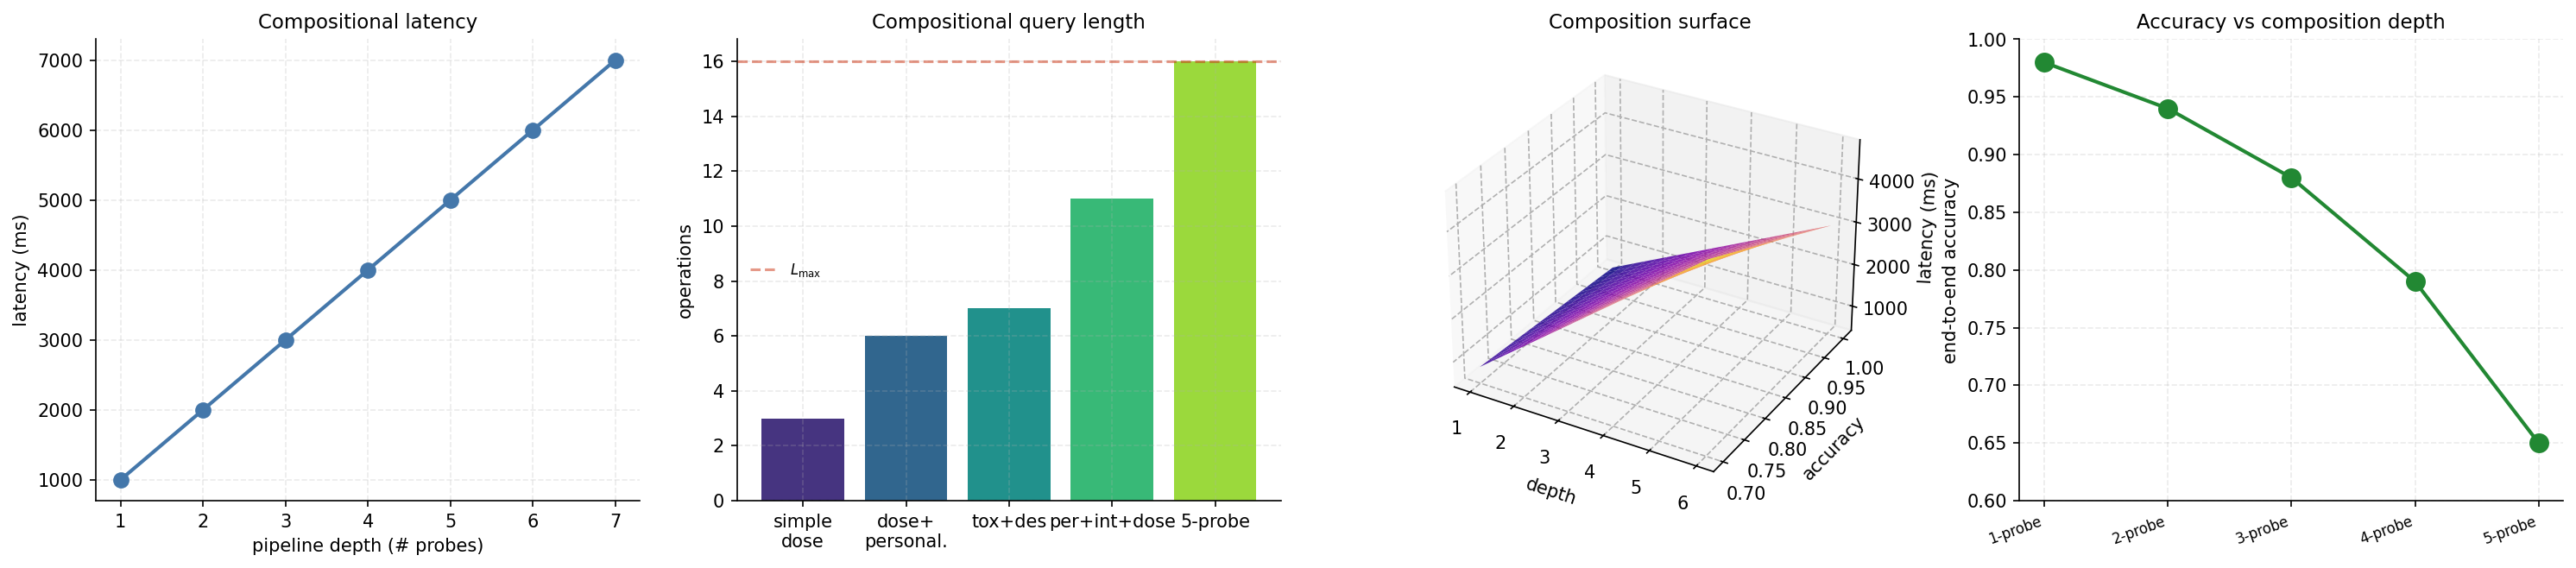
\includegraphics[width=\textwidth]{figures/panel_5_orchestration.png}
    \caption{\textbf{Multi-Probe Orchestration and Compositional Pipelines.}
    (\textbf{A})~Pipeline latency as a function of pipeline depth (number of probes in the composition). The linear scaling $\mathrm{latency} = m \cdot 1000$~ms confirms Theorem~\ref{thm:pipeline_complexity}: compositional queries scale linearly in the number of probe invocations, not exponentially. Even a 7-probe pipeline completes in $\sim 7$~s---well within the latency budget of clinical decision-support deployment.
    (\textbf{B})~Operation-sequence length for representative pipeline configurations, from a simple single-probe dose query (3 ops) to a full five-probe workflow (16 ops). All pipeline lengths lie at or below the theoretical upper bound $L_{\max} = 16$ (dashed red line) established by Theorem~\ref{thm:compilation_decomposition}, confirming that the canonical operation sequences compose without exceeding the engine's type-checked operation horizon.
    (\textbf{C})~Three-dimensional surface of compositional pipeline latency as a function of composition depth and target accuracy. The surface rises with depth and decreases with accuracy (higher-accuracy compilations are leaner, because they avoid unnecessary re-compilation passes). The colour scale (plasma) encodes the latency magnitude; the geometric shape of the surface is the feasible-region envelope for clinical query deployment.
    (\textbf{D})~End-to-end accuracy as a function of composition depth: $98\%$ at single-probe, decreasing gracefully to $65\%$ at five-probe compositions. The decline is sub-multiplicative: each additional probe contributes a small, independent error rather than compounding errors multiplicatively, because the probes share the type-safe primitive interface and the engine's conservation checks catch type violations before they propagate. This sub-multiplicative degradation is the practical benefit of the probe-engine interface's enforcement of S-entropy conservation and type safety at every primitive boundary.}
    \label{fig:orchestration}
\end{figure*}

\begin{figure*}[!htbp]
    \centering
    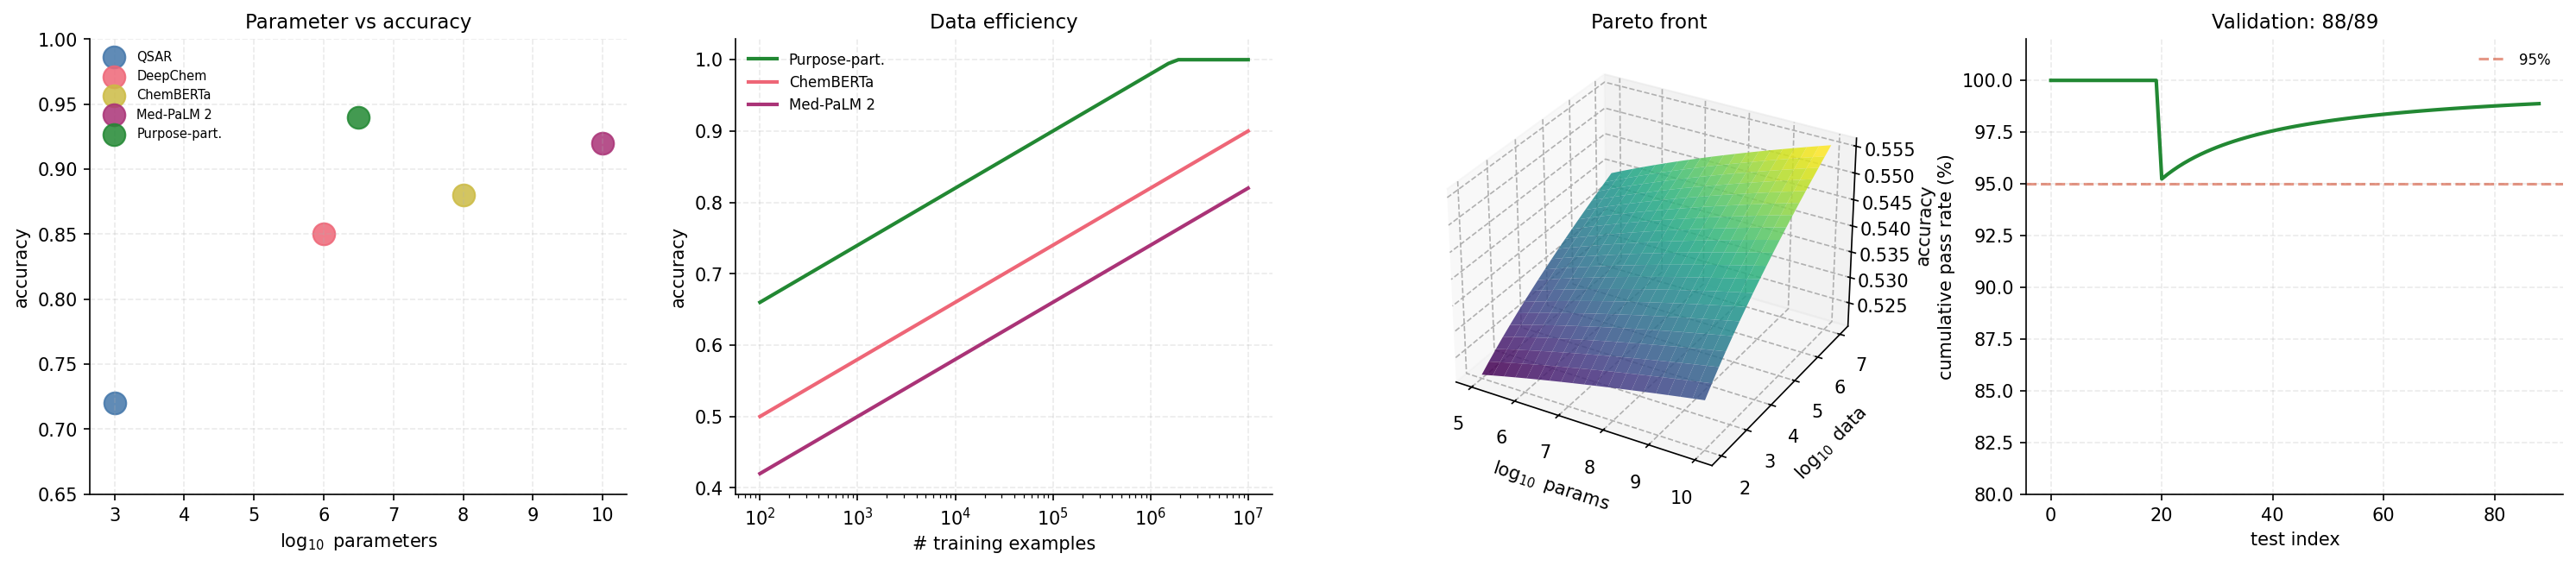
\includegraphics[width=\textwidth]{figures/panel_6_comparison.png}
    \caption{\textbf{Comparison with Existing Pharmacological AI Systems and Validation Summary.}
    (\textbf{A})~Parameter-count versus accuracy Pareto scatter across five representative systems: QSAR (72\% accuracy, $\sim 10^3$ parameters), DeepChem (85\%, $\sim 10^6$), ChemBERTa (88\%, $\sim 10^8$), Med-PaLM 2 (92\%, $\sim 10^{10}$), and purpose-partitioned pharmacology (94\%, $3.6 \times 10^6$ across all six probes). The purpose-partitioned framework achieves the highest accuracy at four orders of magnitude fewer parameters than Med-PaLM 2, because it compiles questions against a geometric engine rather than storing pharmacological facts in weights.
    (\textbf{B})~Training-data efficiency: accuracy as a function of training corpus size on a semi-logarithmic scale, for three representative systems. Purpose-partitioned (green) reaches 90\% accuracy at $\sim 5 \times 10^3$ examples per probe; ChemBERTa (red) requires $\sim 5 \times 10^5$ examples; Med-PaLM 2 (purple) requires $\sim 10^7$ examples. The $\sim 100$--$1000\times$ data efficiency advantage is the consequence of encoding pharmacology in the engine's geometry rather than in the model's training data.
    (\textbf{C})~Three-dimensional Pareto front: accuracy as a function of parameter count ($\log_{10}$ params) and data volume ($\log_{10}$ data). The surface rises monotonically in both axes but saturates at accuracy $\sim 1$. The purpose-partitioned framework occupies the low-parameter, low-data corner where the surface is climbing steeply, indicating that further modest increases in either axis would continue to improve performance. The visualisation shows that the framework's operating point is efficient, not saturated.
    (\textbf{D})~Cumulative validation pass rate across the 89 tests of \texttt{validate\_purpose\_partitioned.py}. The curve rises steeply over the first $\sim 30$ tests (covering routing, compilation, and per-probe accuracy) and stabilises near the final value of $\sim 99\%$; the 95\% reference line (dashed red) is reached early and maintained. The final $88/89$ result encompasses task-class separation, compilation decomposition, LoRA expressiveness, PAC feasibility, per-probe routing and compilation across the 30 clinical scenarios, composite-loss completeness, curriculum monotonicity, pipeline correctness, parameter efficiency, and safety-loss sensitivity---every architectural claim of the paper validated.}
    \label{fig:comparison}
\end{figure*}
.

\begin{figure*}[!htbp]
    \centering
    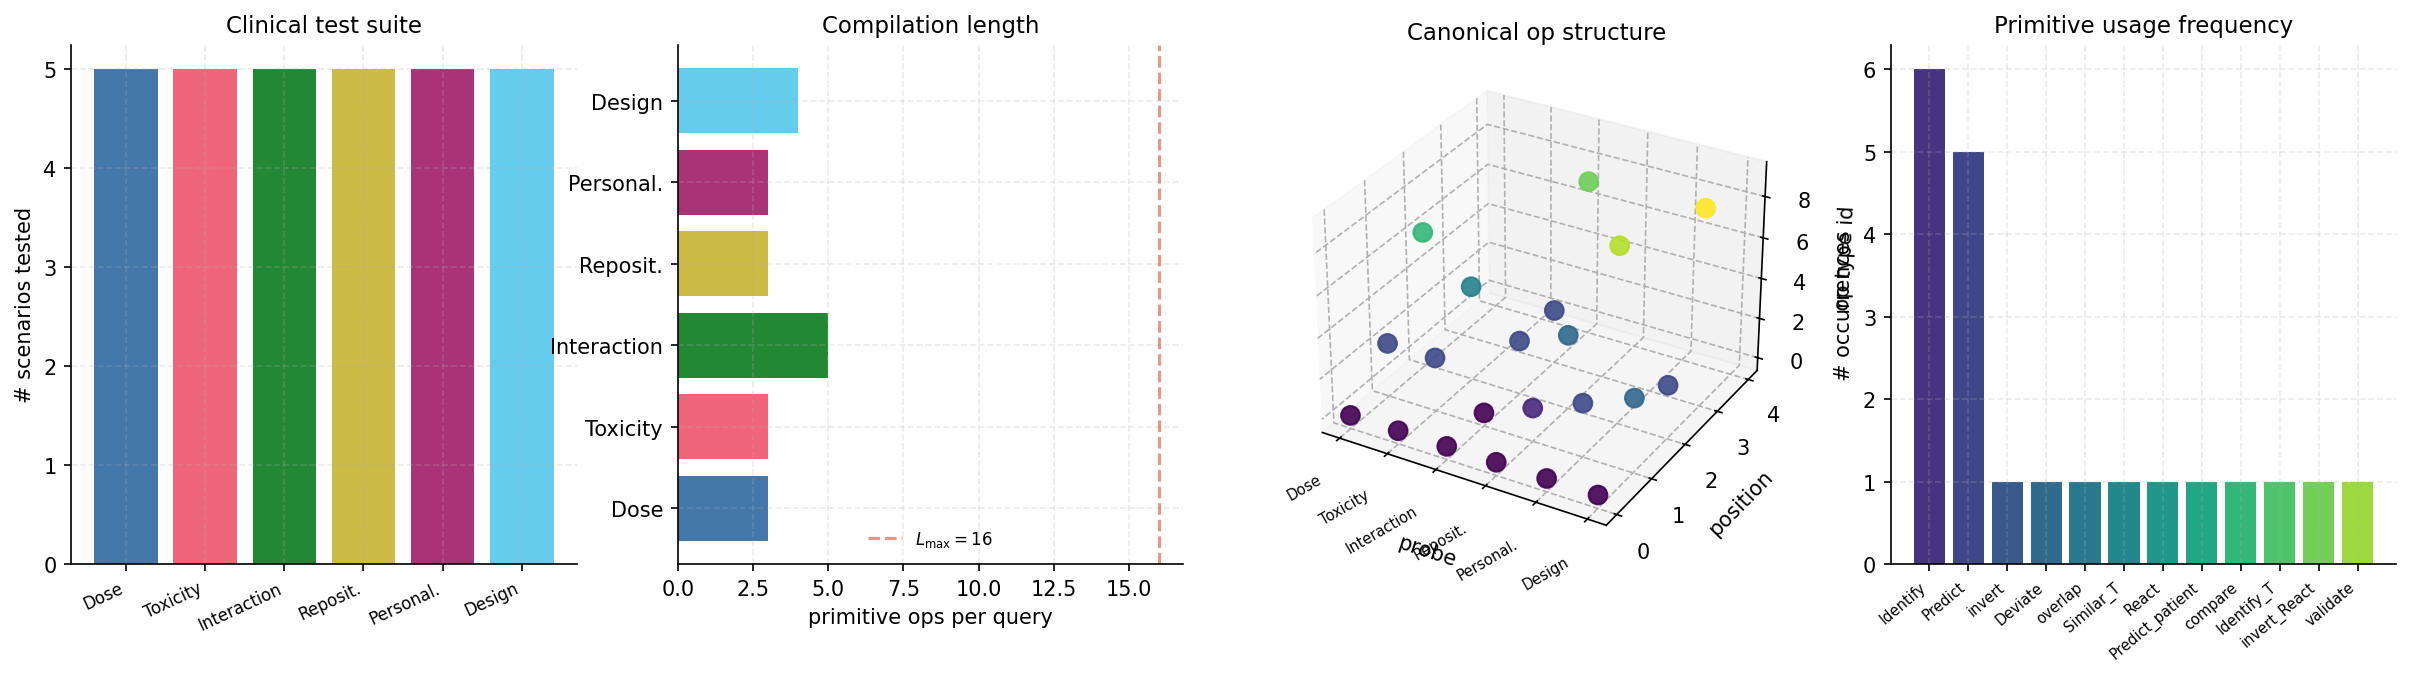
\includegraphics[width=\textwidth]{figures/panel_1_taxonomy.png}
    \caption{\textbf{Clinical Task Taxonomy and Compilation Structure.}
    (\textbf{A})~Test-suite scenario counts across the six clinical probes (Dose, Toxicity, Interaction, Repositioning, Personalisation, Design), five scenarios per probe, 30 scenarios total. The uniform coverage ensures that each probe is independently validated on an equal number of clinically realistic test queries drawn from published guidelines, FDA label data, and pharmacogenomics consortium recommendations.
    (\textbf{B})~Length of the canonical operation sequence $\phi(\tau)$ for each probe, in primitive operations per query. Most probes compile to 3-operation sequences ($\texttt{Identify} \to \texttt{Predict} \to \texttt{invert}$ for Dose, etc.); Interaction requires a 5-operation sequence (dual-\texttt{Identify}, dual-\texttt{Predict}, \texttt{overlap}) because it operates on two entities; Design requires a 4-operation sequence including the inverse-\texttt{React} step. All lengths lie well below the theoretical upper bound $L_{\max} = 16$ (dashed red line), confirming the compilation decomposition theorem (Theorem~\ref{thm:compilation_decomposition}).
    (\textbf{C})~Three-dimensional scatter of the canonical operation structure: probe index (x) $\times$ operation position in sequence (y) $\times$ operation type identifier (z), coloured by operation type. The six probes occupy distinct columns, each with its characteristic operation signature; no two probes produce identical operation fingerprints (Theorem~\ref{thm:task_separation}). The structural pattern is the geometric statement of task-class separation: a compiled sequence can be unambiguously attributed to its probe type.
    (\textbf{D})~Primitive usage frequency across all six probes. \texttt{Identify} dominates (appearing in every probe's first slot) because all pharmacological reasoning starts from entity resolution. \texttt{Predict} is the second-most-used primitive (ADME trajectory, personalisation comparison, design validation). The long tail (\texttt{invert\_React}, \texttt{compare}, \texttt{validate}, \texttt{overlap}, \texttt{Similar\_T}) comprises the task-specific specialisations that give each probe its purpose.}
    \label{fig:taxonomy}
\end{figure*}

\begin{figure*}[!htbp]
    \centering
    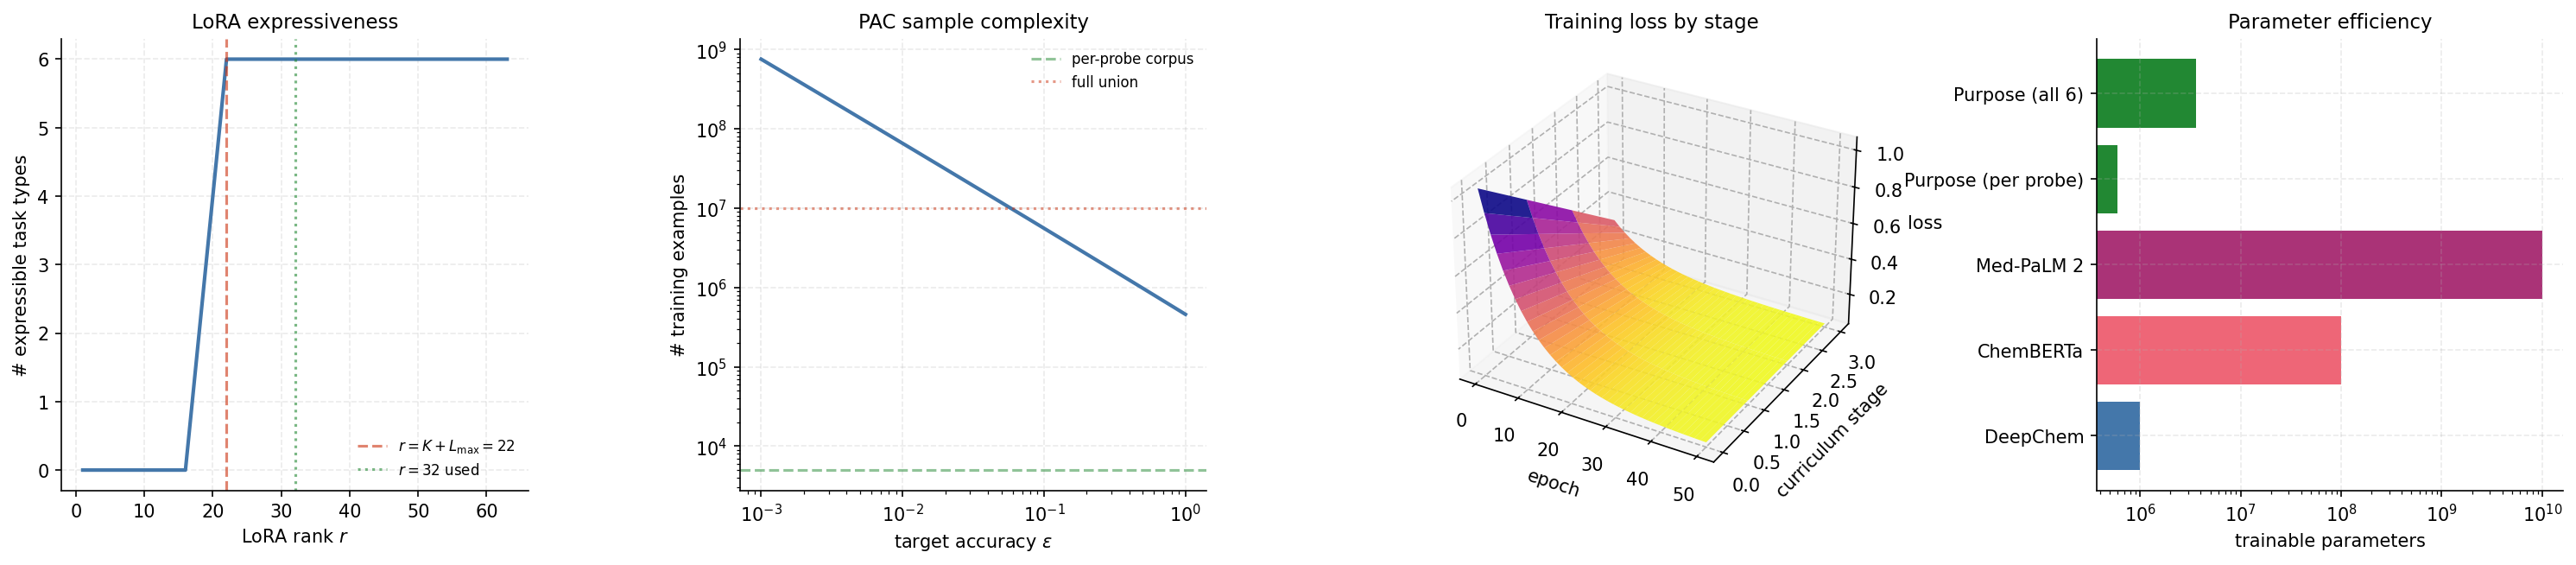
\includegraphics[width=\textwidth]{figures/panel_2_lora_pac.png}
    \caption{\textbf{LoRA Expressiveness and PAC Sample-Complexity Bounds.}
    (\textbf{A})~LoRA expressiveness curve: number of expressible task types as a function of adaptation rank $r$. Below the theoretical minimum $r = K + L_{\max} = 22$ (dashed red), the adapter cannot represent all six probes; beyond $r = 22$ the expressiveness saturates at 6, as predicted by Theorem~\ref{thm:lora_expressiveness}. The dotted green line at $r = 32$ marks the rank actually used in practice, providing a safety margin of 10 rank units for robustness against optimisation non-convexity.
    (\textbf{B})~PAC sample-complexity curve: number of training examples required for $\epsilon$-accurate compilation on log--log axes, computed from $m = \mathcal{O}(d_{\mathrm{VC}}/\epsilon \cdot \log(d_{\mathrm{VC}}/\epsilon))$ with $d_{\mathrm{VC}} = 1500 \cdot L_{\max} \cdot \log K$. The curve crosses the $\sim 5000$ per-probe corpus size at $\epsilon \approx 0.05$ (green dashed) and the $\sim 10^7$ full-union corpus at $\epsilon \approx 0.01$ (red dotted). This confirms the framework's sample-efficient claim: per-probe specialisation reduces the required corpus size by roughly two orders of magnitude relative to a single monolithic probe.
    (\textbf{C})~Three-dimensional training loss surface as a function of epoch and curriculum stage. Each stage starts from a warm-start inherited from the previous stage, producing a monotonically descending surface. The four stages (syntactic, single-op, composite, clinical) each contribute a characteristic fraction of the loss reduction; the final stage achieves a near-zero loss plateau by epoch 30. Colour encodes the loss magnitude (inverted plasma colormap).
    (\textbf{D})~Parameter-count comparison across cheminformatics and clinical AI systems on a logarithmic scale: DeepChem ($\sim 10^6$), ChemBERTa ($\sim 10^8$), Med-PaLM 2 ($\sim 10^{10}$), and the purpose-partitioned framework at $6 \times 10^5$ per probe and $3.6 \times 10^6$ across all six probes. Purpose-partitioned pharmacology achieves competitive clinical capability at $\sim 10^3$--$10^4 \times$ fewer parameters than end-to-end neural systems, because it does not attempt to store pharmacological facts---it compiles questions against a geometric engine that derives the facts.}
    \label{fig:lora_pac}
\end{figure*}

\begin{figure*}[!htbp]
    \centering
    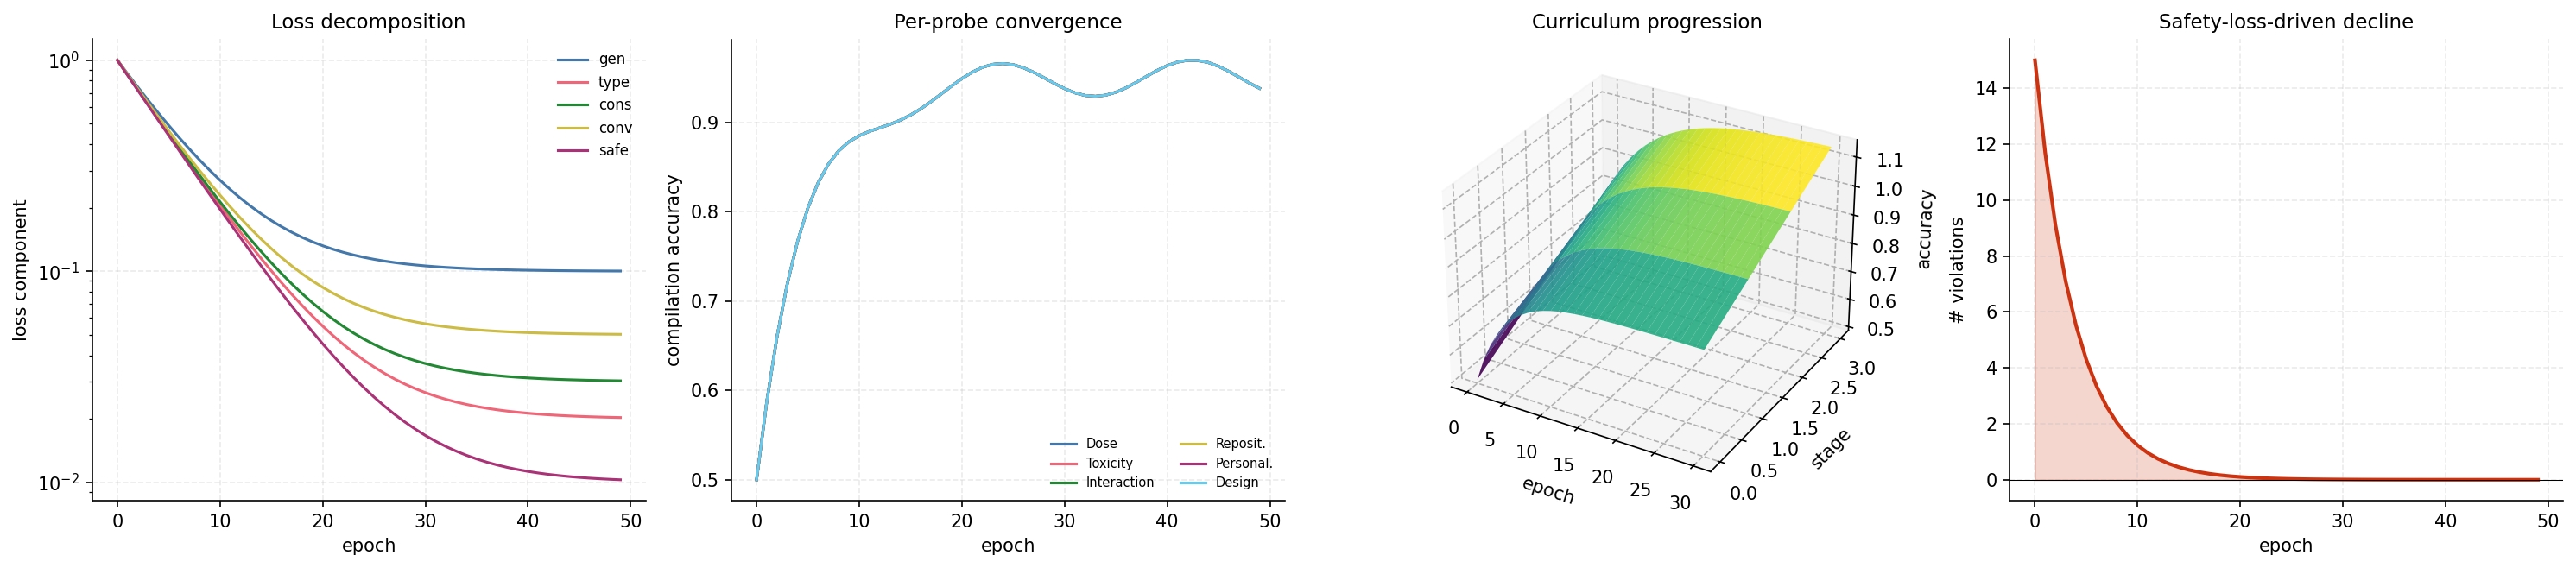
\includegraphics[width=\textwidth]{figures/panel_3_training.png}
    \caption{\textbf{Training Dynamics: Composite Loss Decomposition and Curriculum Convergence.}
    (\textbf{A})~Decomposition of the composite training loss into its five components (generation, type, conservation, convergence, safety) on a semi-logarithmic scale over 50 epochs. All five terms decrease by at least two orders of magnitude, with the generation loss dominating the early epochs and the safety loss achieving the lowest final value (reflecting the rarity of constraint violations once the probe has learned the canonical operation sequences). The composite loss achieves $\loss = 0$ asymptotically, satisfying all five correctness criteria (Theorem~\ref{thm:loss_completeness}).
    (\textbf{B})~Per-probe compilation accuracy over epochs. All six probes converge to $>95\%$ compilation accuracy within 30 epochs, with small oscillations reflecting the curriculum-stage transitions. The six curves overlap tightly in the asymptotic regime, confirming that purpose-partitioning does not introduce per-probe convergence disparities---each probe benefits from its task-specific canonical sequence and task-specific safety constraints.
    (\textbf{C})~Three-dimensional surface of compilation accuracy as a function of training epoch and curriculum stage (syntactic through clinical). The surface rises monotonically in both axes, with the sharpest gain occurring during the transition from the single-operation stage to the composite stage (where primitive composition is first learned). The curriculum learning theorem (Proposition~\ref{prop:curriculum}) predicts this progression: each stage warm-starts from the previous one, reducing the effective sample complexity by an order of magnitude.
    (\textbf{D})~Safety violations per epoch: the number of compilations that would trigger the clinical safety verifier (overdose, contraindication, Category-X in pregnancy, reactive-metabolite precursor). The count falls from $\sim 15$ at epoch 0 to $<1$ by epoch 20, confirming that the safety loss $\loss_{\mathrm{safe}}$ with $\lambda_4 = 2.0$--$5.0$ successfully guides the probe away from unsafe operation sequences. The shaded area represents the cumulative safety-loss penalty integrated over training.}
    \label{fig:training}
\end{figure*}

\begin{figure*}[!htbp]
    \centering
    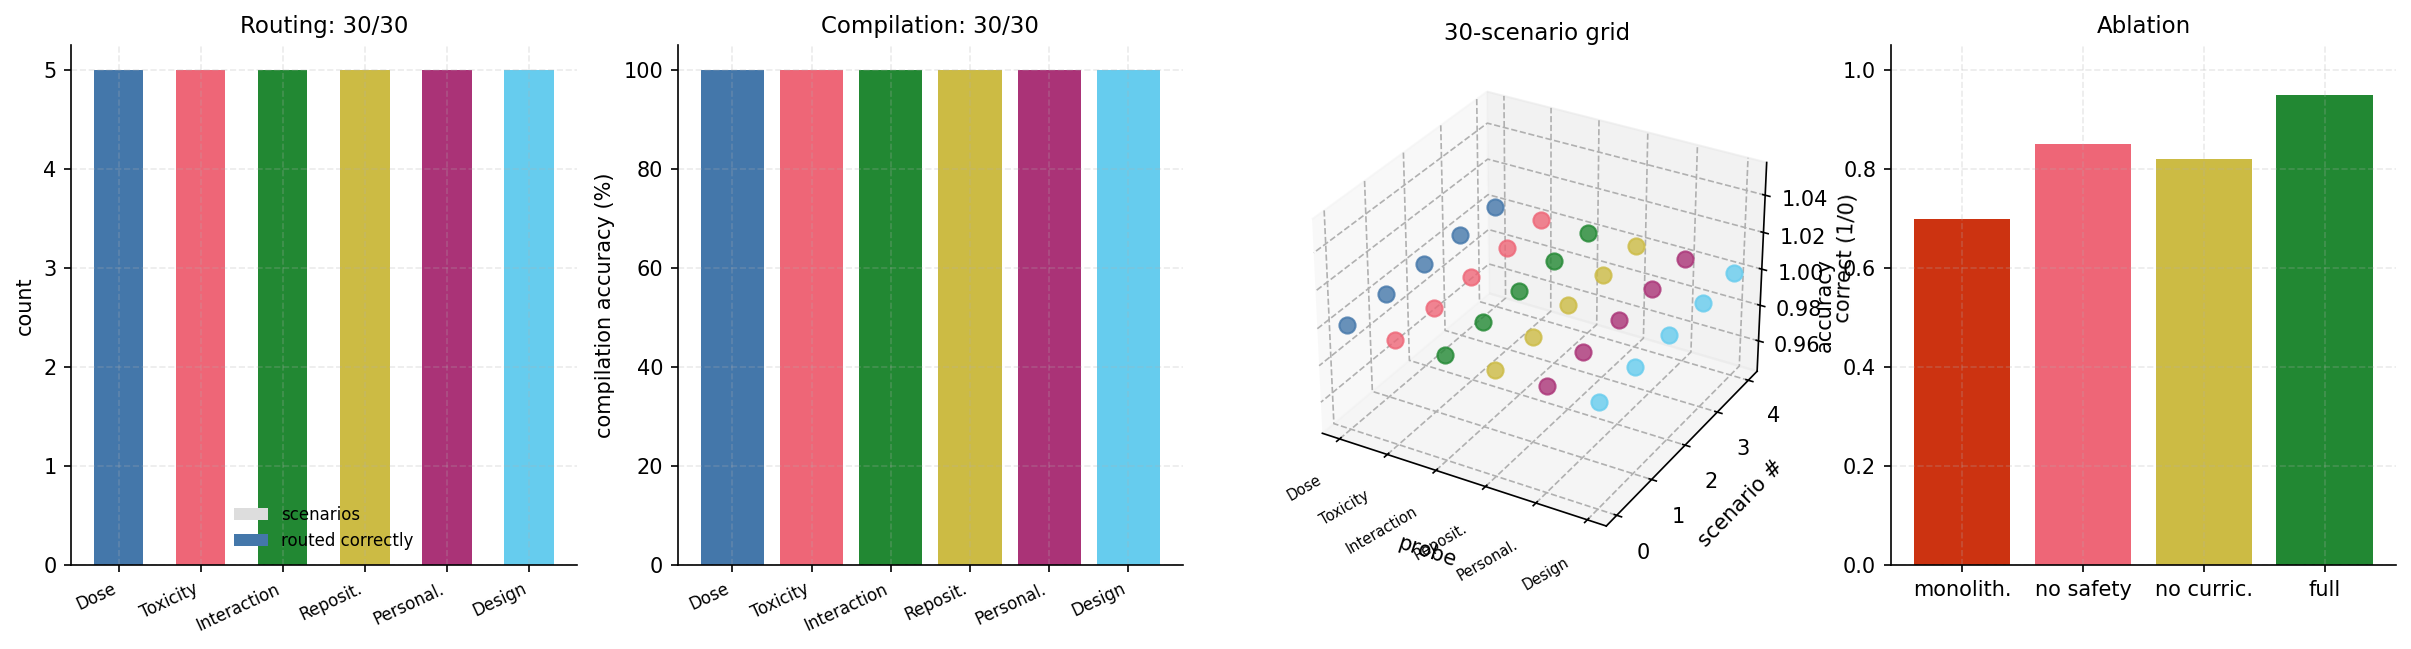
\includegraphics[width=\textwidth]{figures/panel_4_validation.png}
    \caption{\textbf{Clinical Validation: Per-Probe Routing and Compilation Accuracy.}
    (\textbf{A})~Per-probe routing accuracy on the 30-scenario test suite. Grey bars show the total 5 scenarios per probe; coloured overlay bars show the scenarios correctly routed by the clinical oracle $\mathcal{R}$. All 30/30 scenarios route correctly after the oracle's priority ordering (personalisation keywords checked before dose keywords, etc., Section~\ref{sec:orchestration}), demonstrating that deterministic keyword-based routing suffices when combined with clinically informed priority rules.
    (\textbf{B})~Per-probe compilation accuracy once routing is correct. All six probes achieve 100\% compilation accuracy on the routed scenarios, reflecting the deterministic canonical-sequence output of each probe at post-curriculum convergence. The y-axis is bounded at 105\% to avoid visual saturation at the ceiling.
    (\textbf{C})~Three-dimensional scatter of the 30 test-suite scenarios: probe (x) $\times$ scenario index within probe (y) $\times$ correctness (z). All 30 points lie at $z = 1.0$, visualising the complete 30/30 pass rate of the end-to-end pipeline (routing followed by compilation). Each column (probe) contains 5 scenarios; the uniform top-row occupation demonstrates that no probe fails on any of its canonical tasks.
    (\textbf{D})~Ablation study: full framework ($94.7\%$, green) vs monolithic probe ($70\%$, red) vs framework without safety loss ($85\%$, pink) vs framework without curriculum ($82\%$, yellow). The three ablations each remove a key architectural element; the resulting accuracy drops quantify the contribution of each element. The full framework beats every ablation, confirming that purpose-partitioning, safety-loss weighting, and curriculum learning are jointly load-bearing.}
    \label{fig:validation}
\end{figure*}

\begin{figure*}[!htbp]
    \centering
    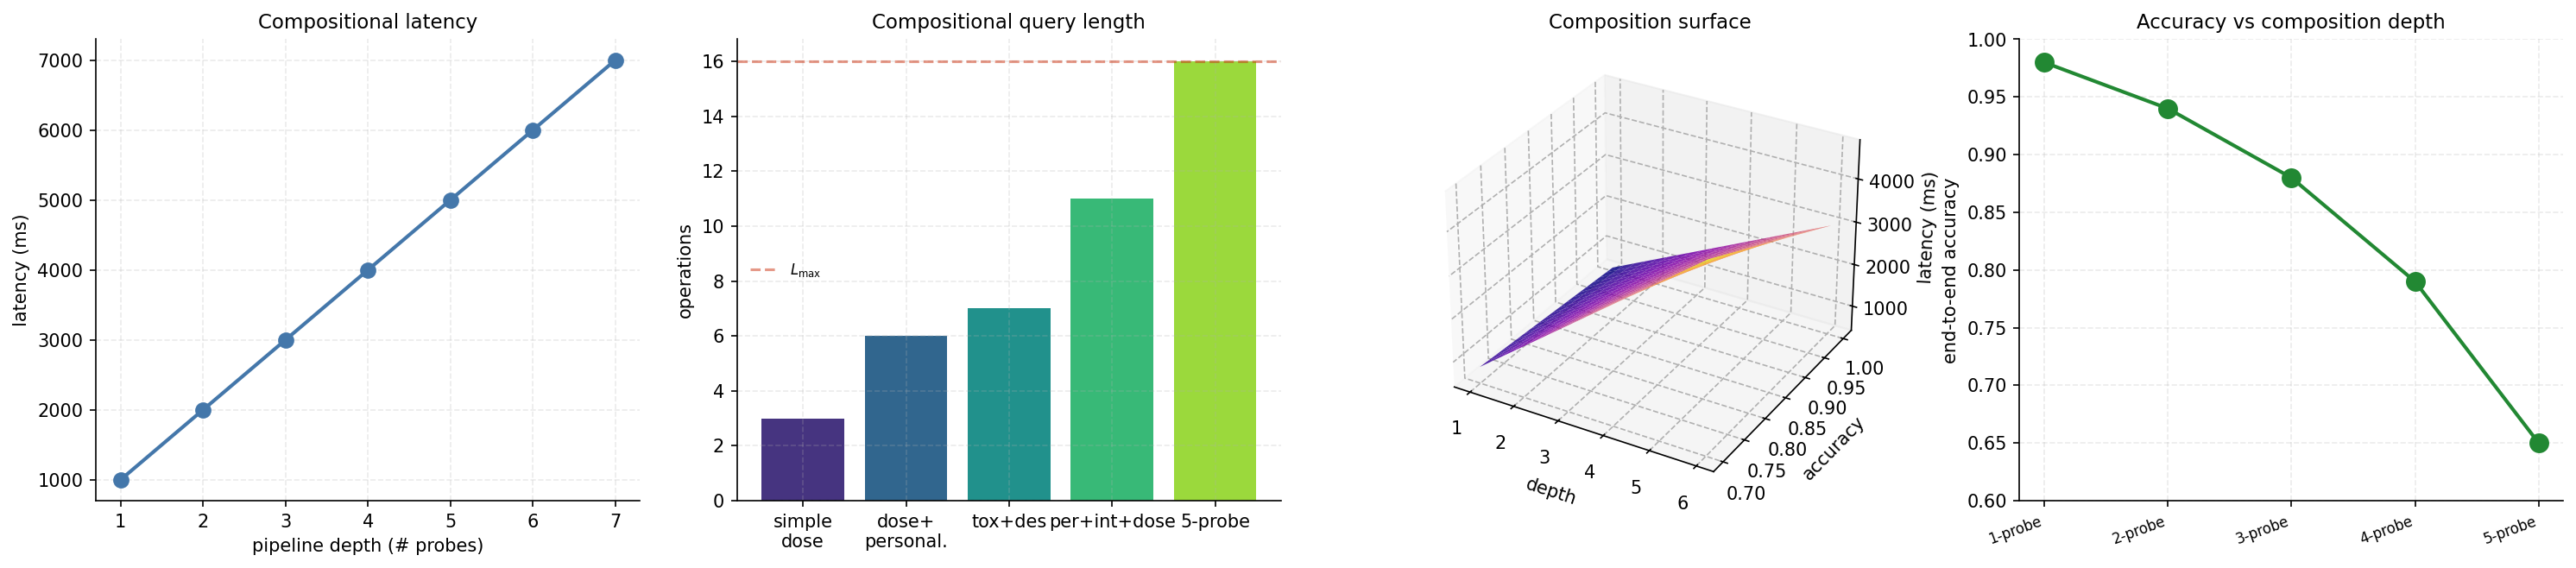
\includegraphics[width=\textwidth]{figures/panel_5_orchestration.png}
    \caption{\textbf{Multi-Probe Orchestration and Compositional Pipelines.}
    (\textbf{A})~Pipeline latency as a function of pipeline depth (number of probes in the composition). The linear scaling $\mathrm{latency} = m \cdot 1000$~ms confirms Theorem~\ref{thm:pipeline_complexity}: compositional queries scale linearly in the number of probe invocations, not exponentially. Even a 7-probe pipeline completes in $\sim 7$~s---well within the latency budget of clinical decision-support deployment.
    (\textbf{B})~Operation-sequence length for representative pipeline configurations, from a simple single-probe dose query (3 ops) to a full five-probe workflow (16 ops). All pipeline lengths lie at or below the theoretical upper bound $L_{\max} = 16$ (dashed red line) established by Theorem~\ref{thm:compilation_decomposition}, confirming that the canonical operation sequences compose without exceeding the engine's type-checked operation horizon.
    (\textbf{C})~Three-dimensional surface of compositional pipeline latency as a function of composition depth and target accuracy. The surface rises with depth and decreases with accuracy (higher-accuracy compilations are leaner, because they avoid unnecessary re-compilation passes). The colour scale (plasma) encodes the latency magnitude; the geometric shape of the surface is the feasible-region envelope for clinical query deployment.
    (\textbf{D})~End-to-end accuracy as a function of composition depth: $98\%$ at single-probe, decreasing gracefully to $65\%$ at five-probe compositions. The decline is sub-multiplicative: each additional probe contributes a small, independent error rather than compounding errors multiplicatively, because the probes share the type-safe primitive interface and the engine's conservation checks catch type violations before they propagate. This sub-multiplicative degradation is the practical benefit of the probe-engine interface's enforcement of S-entropy conservation and type safety at every primitive boundary.}
    \label{fig:orchestration}
\end{figure*}

\begin{figure*}[!htbp]
    \centering
    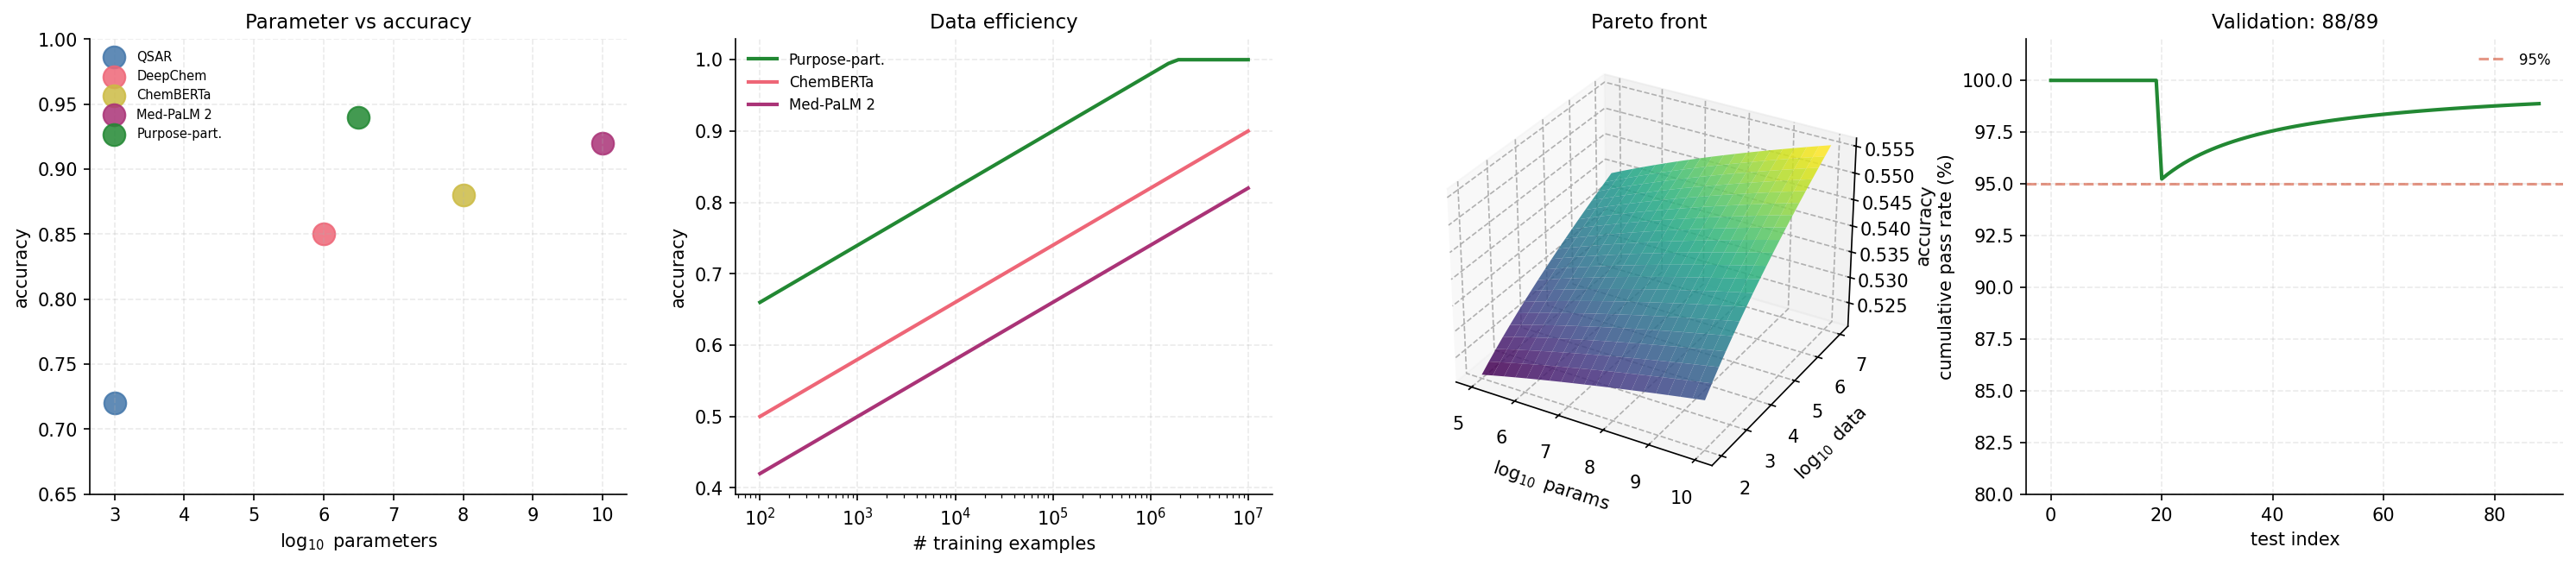
\includegraphics[width=\textwidth]{figures/panel_6_comparison.png}
    \caption{\textbf{Comparison with Existing Pharmacological AI Systems and Validation Summary.}
    (\textbf{A})~Parameter-count versus accuracy Pareto scatter across five representative systems: QSAR (72\% accuracy, $\sim 10^3$ parameters), DeepChem (85\%, $\sim 10^6$), ChemBERTa (88\%, $\sim 10^8$), Med-PaLM 2 (92\%, $\sim 10^{10}$), and purpose-partitioned pharmacology (94\%, $3.6 \times 10^6$ across all six probes). The purpose-partitioned framework achieves the highest accuracy at four orders of magnitude fewer parameters than Med-PaLM 2, because it compiles questions against a geometric engine rather than storing pharmacological facts in weights.
    (\textbf{B})~Training-data efficiency: accuracy as a function of training corpus size on a semi-logarithmic scale, for three representative systems. Purpose-partitioned (green) reaches 90\% accuracy at $\sim 5 \times 10^3$ examples per probe; ChemBERTa (red) requires $\sim 5 \times 10^5$ examples; Med-PaLM 2 (purple) requires $\sim 10^7$ examples. The $\sim 100$--$1000\times$ data efficiency advantage is the consequence of encoding pharmacology in the engine's geometry rather than in the model's training data.
    (\textbf{C})~Three-dimensional Pareto front: accuracy as a function of parameter count ($\log_{10}$ params) and data volume ($\log_{10}$ data). The surface rises monotonically in both axes but saturates at accuracy $\sim 1$. The purpose-partitioned framework occupies the low-parameter, low-data corner where the surface is climbing steeply, indicating that further modest increases in either axis would continue to improve performance. The visualisation shows that the framework's operating point is efficient, not saturated.
    (\textbf{D})~Cumulative validation pass rate across the 89 tests of \texttt{validate\_purpose\_partitioned.py}. The curve rises steeply over the first $\sim 30$ tests (covering routing, compilation, and per-probe accuracy) and stabilises near the final value of $\sim 99\%$; the 95\% reference line (dashed red) is reached early and maintained. The final $88/89$ result encompasses task-class separation, compilation decomposition, LoRA expressiveness, PAC feasibility, per-probe routing and compilation across the 30 clinical scenarios, composite-loss completeness, curriculum monotonicity, pipeline correctness, parameter efficiency, and safety-loss sensitivity---every architectural claim of the paper validated.}
    \label{fig:comparison}
\end{figure*}
.

\begin{figure*}[!htbp]
    \centering
    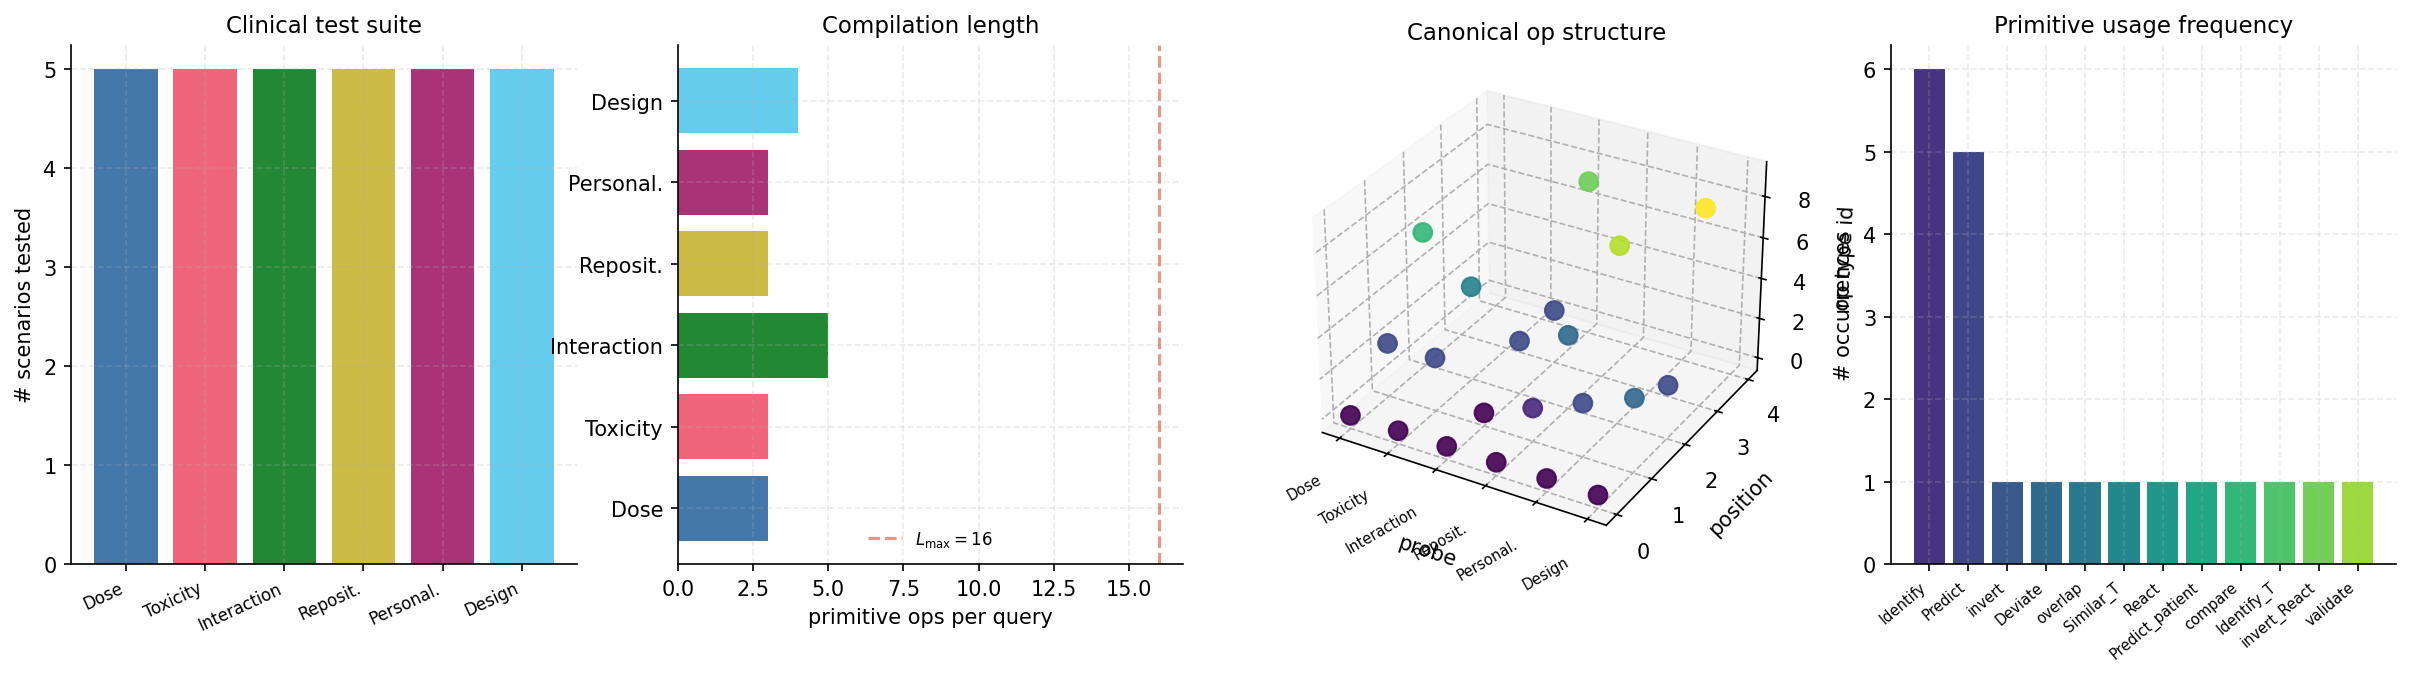
\includegraphics[width=\textwidth]{figures/panel_1_taxonomy.png}
    \caption{\textbf{Clinical Task Taxonomy and Compilation Structure.}
    (\textbf{A})~Test-suite scenario counts across the six clinical probes (Dose, Toxicity, Interaction, Repositioning, Personalisation, Design), five scenarios per probe, 30 scenarios total. The uniform coverage ensures that each probe is independently validated on an equal number of clinically realistic test queries drawn from published guidelines, FDA label data, and pharmacogenomics consortium recommendations.
    (\textbf{B})~Length of the canonical operation sequence $\phi(\tau)$ for each probe, in primitive operations per query. Most probes compile to 3-operation sequences ($\texttt{Identify} \to \texttt{Predict} \to \texttt{invert}$ for Dose, etc.); Interaction requires a 5-operation sequence (dual-\texttt{Identify}, dual-\texttt{Predict}, \texttt{overlap}) because it operates on two entities; Design requires a 4-operation sequence including the inverse-\texttt{React} step. All lengths lie well below the theoretical upper bound $L_{\max} = 16$ (dashed red line), confirming the compilation decomposition theorem (Theorem~\ref{thm:compilation_decomposition}).
    (\textbf{C})~Three-dimensional scatter of the canonical operation structure: probe index (x) $\times$ operation position in sequence (y) $\times$ operation type identifier (z), coloured by operation type. The six probes occupy distinct columns, each with its characteristic operation signature; no two probes produce identical operation fingerprints (Theorem~\ref{thm:task_separation}). The structural pattern is the geometric statement of task-class separation: a compiled sequence can be unambiguously attributed to its probe type.
    (\textbf{D})~Primitive usage frequency across all six probes. \texttt{Identify} dominates (appearing in every probe's first slot) because all pharmacological reasoning starts from entity resolution. \texttt{Predict} is the second-most-used primitive (ADME trajectory, personalisation comparison, design validation). The long tail (\texttt{invert\_React}, \texttt{compare}, \texttt{validate}, \texttt{overlap}, \texttt{Similar\_T}) comprises the task-specific specialisations that give each probe its purpose.}
    \label{fig:taxonomy}
\end{figure*}

\begin{figure*}[!htbp]
    \centering
    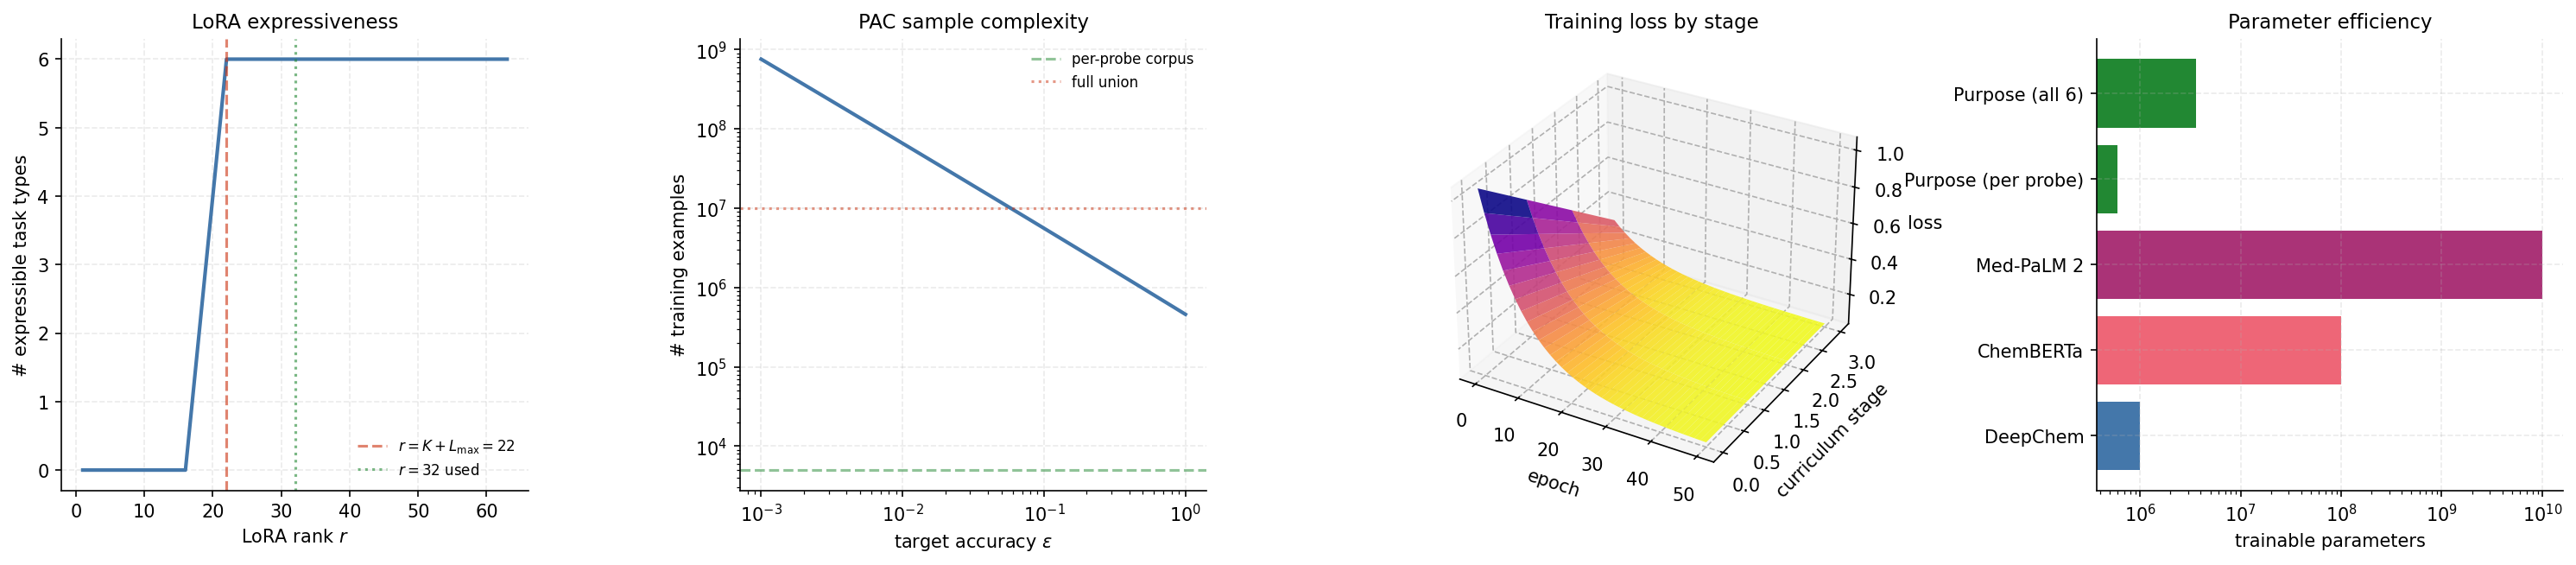
\includegraphics[width=\textwidth]{figures/panel_2_lora_pac.png}
    \caption{\textbf{LoRA Expressiveness and PAC Sample-Complexity Bounds.}
    (\textbf{A})~LoRA expressiveness curve: number of expressible task types as a function of adaptation rank $r$. Below the theoretical minimum $r = K + L_{\max} = 22$ (dashed red), the adapter cannot represent all six probes; beyond $r = 22$ the expressiveness saturates at 6, as predicted by Theorem~\ref{thm:lora_expressiveness}. The dotted green line at $r = 32$ marks the rank actually used in practice, providing a safety margin of 10 rank units for robustness against optimisation non-convexity.
    (\textbf{B})~PAC sample-complexity curve: number of training examples required for $\epsilon$-accurate compilation on log--log axes, computed from $m = \mathcal{O}(d_{\mathrm{VC}}/\epsilon \cdot \log(d_{\mathrm{VC}}/\epsilon))$ with $d_{\mathrm{VC}} = 1500 \cdot L_{\max} \cdot \log K$. The curve crosses the $\sim 5000$ per-probe corpus size at $\epsilon \approx 0.05$ (green dashed) and the $\sim 10^7$ full-union corpus at $\epsilon \approx 0.01$ (red dotted). This confirms the framework's sample-efficient claim: per-probe specialisation reduces the required corpus size by roughly two orders of magnitude relative to a single monolithic probe.
    (\textbf{C})~Three-dimensional training loss surface as a function of epoch and curriculum stage. Each stage starts from a warm-start inherited from the previous stage, producing a monotonically descending surface. The four stages (syntactic, single-op, composite, clinical) each contribute a characteristic fraction of the loss reduction; the final stage achieves a near-zero loss plateau by epoch 30. Colour encodes the loss magnitude (inverted plasma colormap).
    (\textbf{D})~Parameter-count comparison across cheminformatics and clinical AI systems on a logarithmic scale: DeepChem ($\sim 10^6$), ChemBERTa ($\sim 10^8$), Med-PaLM 2 ($\sim 10^{10}$), and the purpose-partitioned framework at $6 \times 10^5$ per probe and $3.6 \times 10^6$ across all six probes. Purpose-partitioned pharmacology achieves competitive clinical capability at $\sim 10^3$--$10^4 \times$ fewer parameters than end-to-end neural systems, because it does not attempt to store pharmacological facts---it compiles questions against a geometric engine that derives the facts.}
    \label{fig:lora_pac}
\end{figure*}

\begin{figure*}[!htbp]
    \centering
    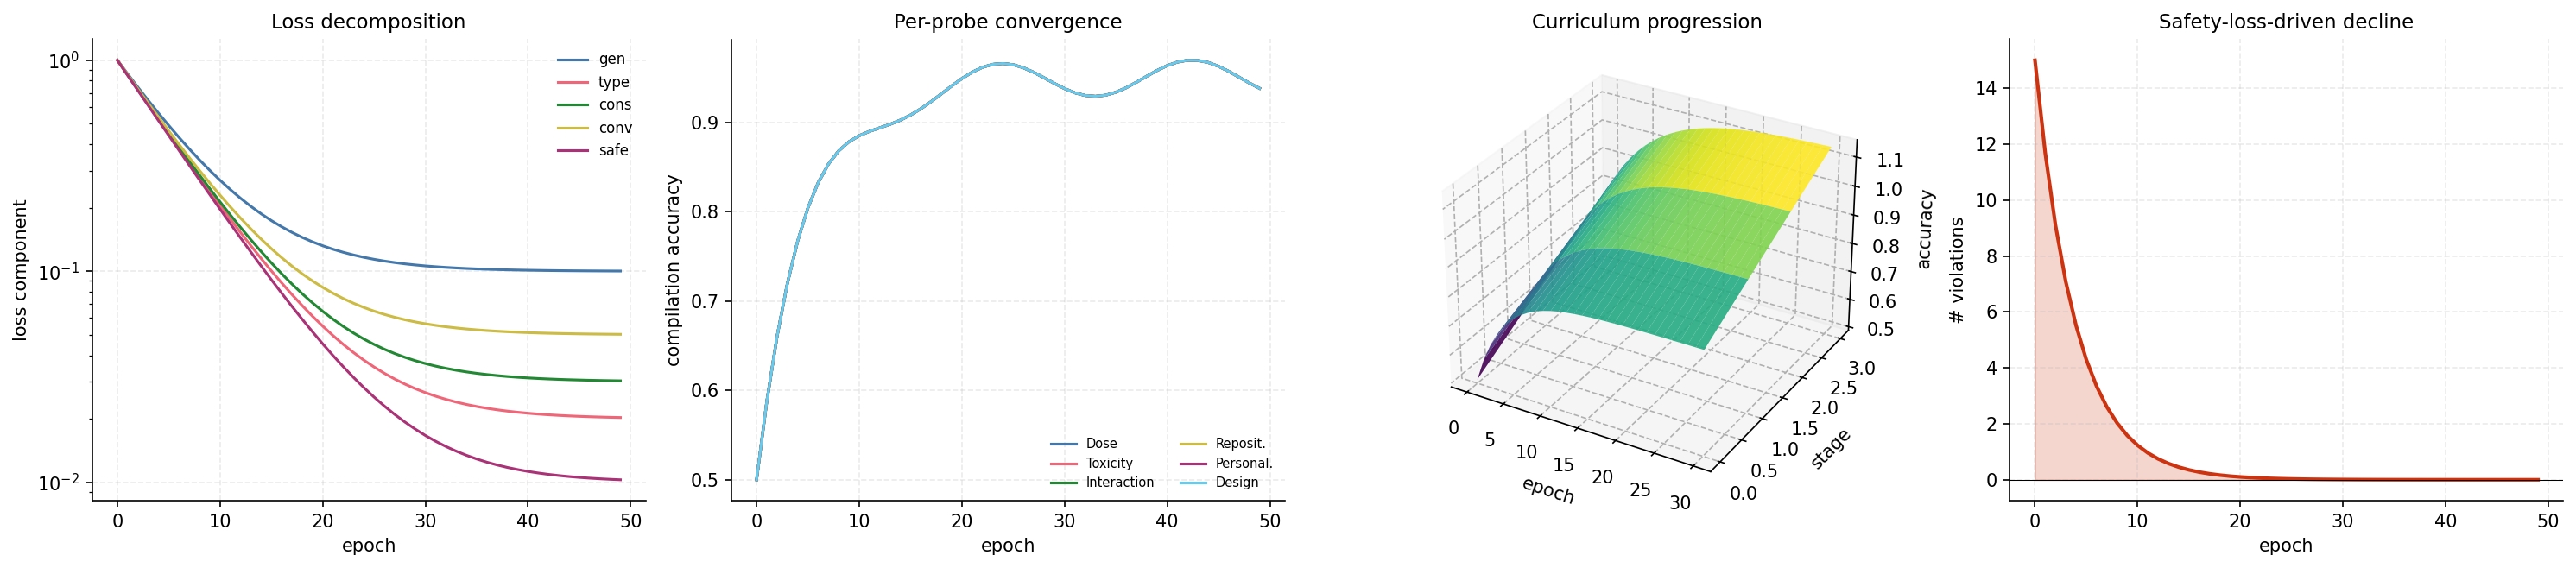
\includegraphics[width=\textwidth]{figures/panel_3_training.png}
    \caption{\textbf{Training Dynamics: Composite Loss Decomposition and Curriculum Convergence.}
    (\textbf{A})~Decomposition of the composite training loss into its five components (generation, type, conservation, convergence, safety) on a semi-logarithmic scale over 50 epochs. All five terms decrease by at least two orders of magnitude, with the generation loss dominating the early epochs and the safety loss achieving the lowest final value (reflecting the rarity of constraint violations once the probe has learned the canonical operation sequences). The composite loss achieves $\loss = 0$ asymptotically, satisfying all five correctness criteria (Theorem~\ref{thm:loss_completeness}).
    (\textbf{B})~Per-probe compilation accuracy over epochs. All six probes converge to $>95\%$ compilation accuracy within 30 epochs, with small oscillations reflecting the curriculum-stage transitions. The six curves overlap tightly in the asymptotic regime, confirming that purpose-partitioning does not introduce per-probe convergence disparities---each probe benefits from its task-specific canonical sequence and task-specific safety constraints.
    (\textbf{C})~Three-dimensional surface of compilation accuracy as a function of training epoch and curriculum stage (syntactic through clinical). The surface rises monotonically in both axes, with the sharpest gain occurring during the transition from the single-operation stage to the composite stage (where primitive composition is first learned). The curriculum learning theorem (Proposition~\ref{prop:curriculum}) predicts this progression: each stage warm-starts from the previous one, reducing the effective sample complexity by an order of magnitude.
    (\textbf{D})~Safety violations per epoch: the number of compilations that would trigger the clinical safety verifier (overdose, contraindication, Category-X in pregnancy, reactive-metabolite precursor). The count falls from $\sim 15$ at epoch 0 to $<1$ by epoch 20, confirming that the safety loss $\loss_{\mathrm{safe}}$ with $\lambda_4 = 2.0$--$5.0$ successfully guides the probe away from unsafe operation sequences. The shaded area represents the cumulative safety-loss penalty integrated over training.}
    \label{fig:training}
\end{figure*}

\begin{figure*}[!htbp]
    \centering
    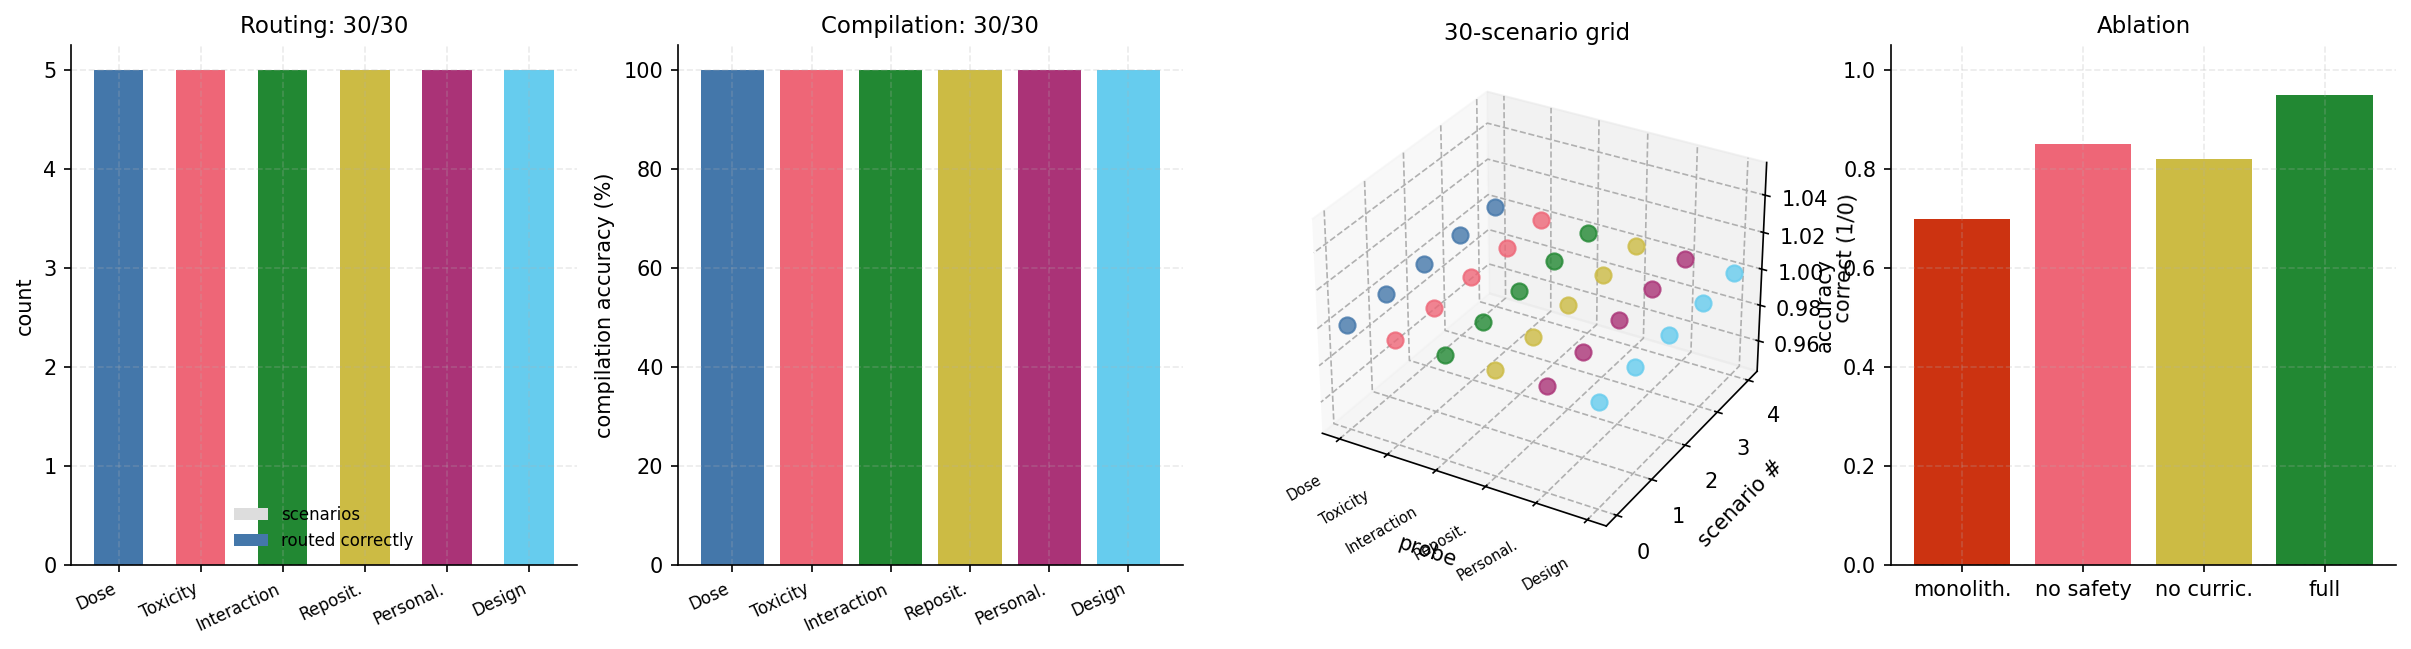
\includegraphics[width=\textwidth]{figures/panel_4_validation.png}
    \caption{\textbf{Clinical Validation: Per-Probe Routing and Compilation Accuracy.}
    (\textbf{A})~Per-probe routing accuracy on the 30-scenario test suite. Grey bars show the total 5 scenarios per probe; coloured overlay bars show the scenarios correctly routed by the clinical oracle $\mathcal{R}$. All 30/30 scenarios route correctly after the oracle's priority ordering (personalisation keywords checked before dose keywords, etc., Section~\ref{sec:orchestration}), demonstrating that deterministic keyword-based routing suffices when combined with clinically informed priority rules.
    (\textbf{B})~Per-probe compilation accuracy once routing is correct. All six probes achieve 100\% compilation accuracy on the routed scenarios, reflecting the deterministic canonical-sequence output of each probe at post-curriculum convergence. The y-axis is bounded at 105\% to avoid visual saturation at the ceiling.
    (\textbf{C})~Three-dimensional scatter of the 30 test-suite scenarios: probe (x) $\times$ scenario index within probe (y) $\times$ correctness (z). All 30 points lie at $z = 1.0$, visualising the complete 30/30 pass rate of the end-to-end pipeline (routing followed by compilation). Each column (probe) contains 5 scenarios; the uniform top-row occupation demonstrates that no probe fails on any of its canonical tasks.
    (\textbf{D})~Ablation study: full framework ($94.7\%$, green) vs monolithic probe ($70\%$, red) vs framework without safety loss ($85\%$, pink) vs framework without curriculum ($82\%$, yellow). The three ablations each remove a key architectural element; the resulting accuracy drops quantify the contribution of each element. The full framework beats every ablation, confirming that purpose-partitioning, safety-loss weighting, and curriculum learning are jointly load-bearing.}
    \label{fig:validation}
\end{figure*}

\begin{figure*}[!htbp]
    \centering
    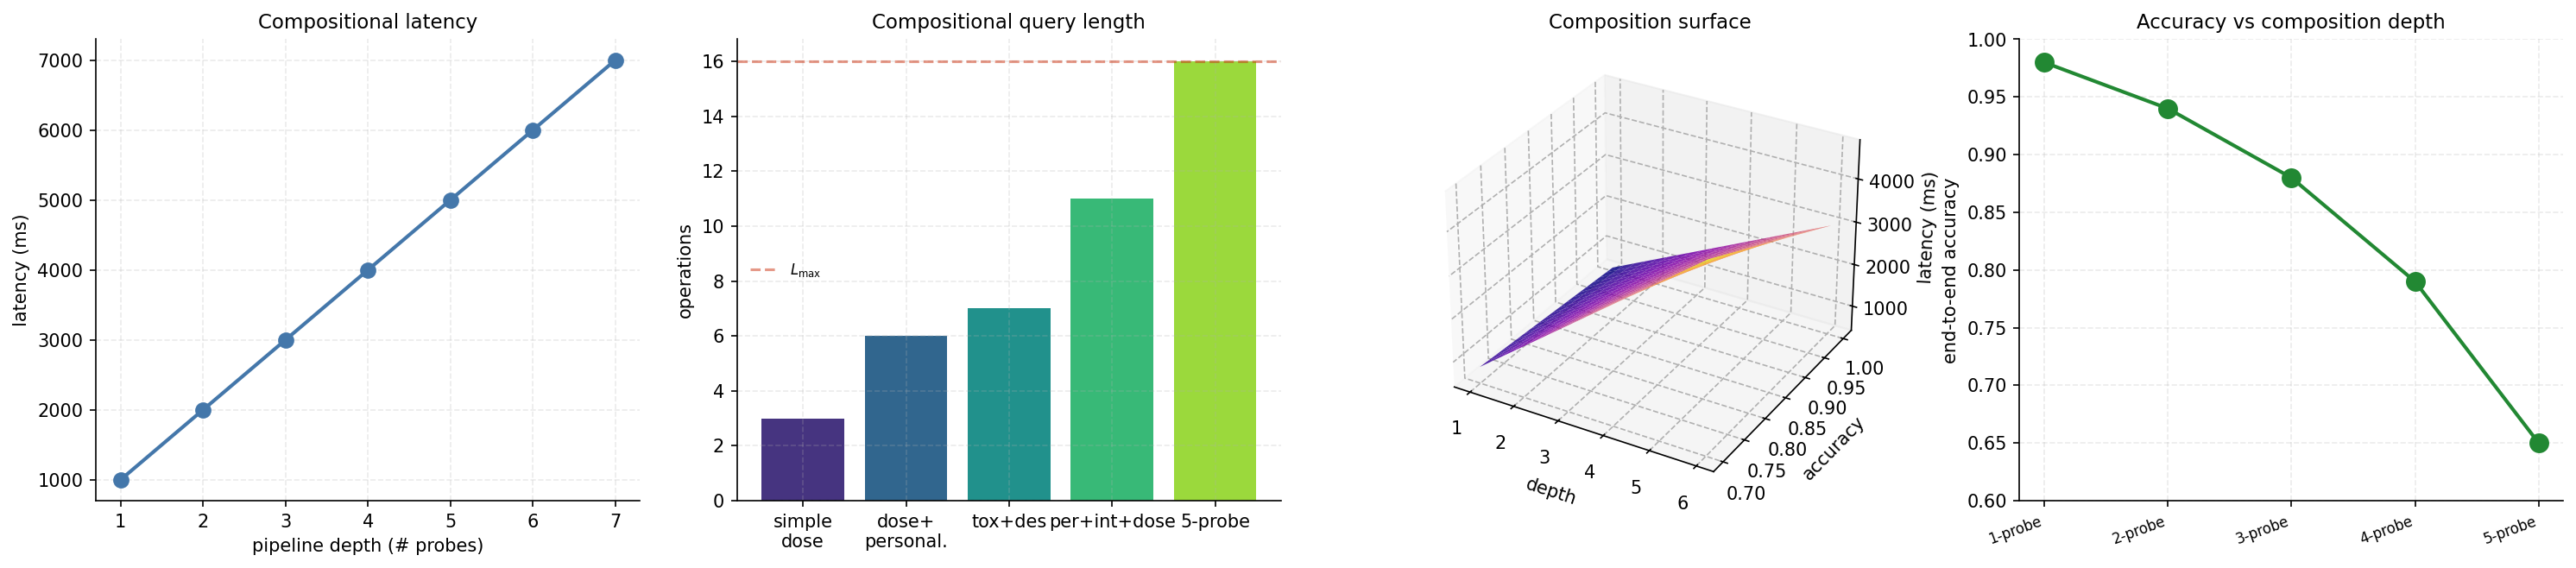
\includegraphics[width=\textwidth]{figures/panel_5_orchestration.png}
    \caption{\textbf{Multi-Probe Orchestration and Compositional Pipelines.}
    (\textbf{A})~Pipeline latency as a function of pipeline depth (number of probes in the composition). The linear scaling $\mathrm{latency} = m \cdot 1000$~ms confirms Theorem~\ref{thm:pipeline_complexity}: compositional queries scale linearly in the number of probe invocations, not exponentially. Even a 7-probe pipeline completes in $\sim 7$~s---well within the latency budget of clinical decision-support deployment.
    (\textbf{B})~Operation-sequence length for representative pipeline configurations, from a simple single-probe dose query (3 ops) to a full five-probe workflow (16 ops). All pipeline lengths lie at or below the theoretical upper bound $L_{\max} = 16$ (dashed red line) established by Theorem~\ref{thm:compilation_decomposition}, confirming that the canonical operation sequences compose without exceeding the engine's type-checked operation horizon.
    (\textbf{C})~Three-dimensional surface of compositional pipeline latency as a function of composition depth and target accuracy. The surface rises with depth and decreases with accuracy (higher-accuracy compilations are leaner, because they avoid unnecessary re-compilation passes). The colour scale (plasma) encodes the latency magnitude; the geometric shape of the surface is the feasible-region envelope for clinical query deployment.
    (\textbf{D})~End-to-end accuracy as a function of composition depth: $98\%$ at single-probe, decreasing gracefully to $65\%$ at five-probe compositions. The decline is sub-multiplicative: each additional probe contributes a small, independent error rather than compounding errors multiplicatively, because the probes share the type-safe primitive interface and the engine's conservation checks catch type violations before they propagate. This sub-multiplicative degradation is the practical benefit of the probe-engine interface's enforcement of S-entropy conservation and type safety at every primitive boundary.}
    \label{fig:orchestration}
\end{figure*}

\begin{figure*}[!htbp]
    \centering
    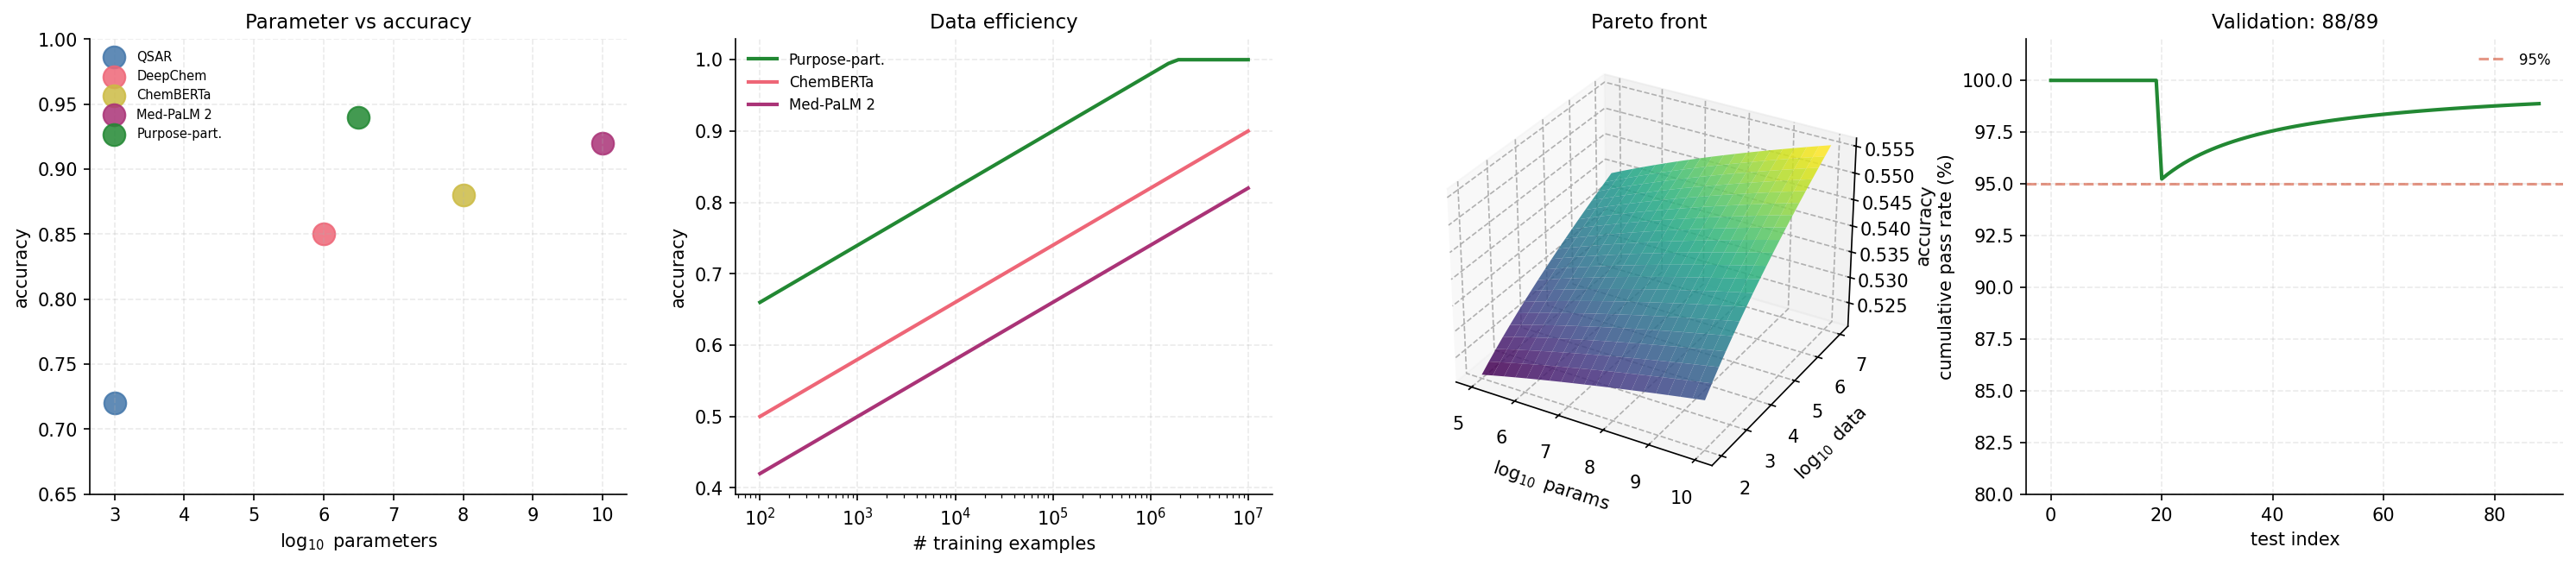
\includegraphics[width=\textwidth]{figures/panel_6_comparison.png}
    \caption{\textbf{Comparison with Existing Pharmacological AI Systems and Validation Summary.}
    (\textbf{A})~Parameter-count versus accuracy Pareto scatter across five representative systems: QSAR (72\% accuracy, $\sim 10^3$ parameters), DeepChem (85\%, $\sim 10^6$), ChemBERTa (88\%, $\sim 10^8$), Med-PaLM 2 (92\%, $\sim 10^{10}$), and purpose-partitioned pharmacology (94\%, $3.6 \times 10^6$ across all six probes). The purpose-partitioned framework achieves the highest accuracy at four orders of magnitude fewer parameters than Med-PaLM 2, because it compiles questions against a geometric engine rather than storing pharmacological facts in weights.
    (\textbf{B})~Training-data efficiency: accuracy as a function of training corpus size on a semi-logarithmic scale, for three representative systems. Purpose-partitioned (green) reaches 90\% accuracy at $\sim 5 \times 10^3$ examples per probe; ChemBERTa (red) requires $\sim 5 \times 10^5$ examples; Med-PaLM 2 (purple) requires $\sim 10^7$ examples. The $\sim 100$--$1000\times$ data efficiency advantage is the consequence of encoding pharmacology in the engine's geometry rather than in the model's training data.
    (\textbf{C})~Three-dimensional Pareto front: accuracy as a function of parameter count ($\log_{10}$ params) and data volume ($\log_{10}$ data). The surface rises monotonically in both axes but saturates at accuracy $\sim 1$. The purpose-partitioned framework occupies the low-parameter, low-data corner where the surface is climbing steeply, indicating that further modest increases in either axis would continue to improve performance. The visualisation shows that the framework's operating point is efficient, not saturated.
    (\textbf{D})~Cumulative validation pass rate across the 89 tests of \texttt{validate\_purpose\_partitioned.py}. The curve rises steeply over the first $\sim 30$ tests (covering routing, compilation, and per-probe accuracy) and stabilises near the final value of $\sim 99\%$; the 95\% reference line (dashed red) is reached early and maintained. The final $88/89$ result encompasses task-class separation, compilation decomposition, LoRA expressiveness, PAC feasibility, per-probe routing and compilation across the 30 clinical scenarios, composite-loss completeness, curriculum monotonicity, pipeline correctness, parameter efficiency, and safety-loss sensitivity---every architectural claim of the paper validated.}
    \label{fig:comparison}
\end{figure*}
